
\documentclass{article} % For LaTeX2e
\usepackage{iclr2026_conference,times}
\usepackage{booktabs}
\usepackage{tabularx}
\usepackage{graphicx}
\usepackage{caption}
\usepackage{subcaption}
\usepackage{threeparttable}
\usepackage{multirow}
\usepackage[ruled,vlined]{algorithm2e}
\usepackage{appendix}
\usepackage{amsmath,amssymb}
\usepackage{wrapfig}
\usepackage{titlesec,titletoc} % titletoc 提供局部目录
\usepackage{xcolor}         % colors
\usepackage[most]{tcolorbox} % 
\usepackage{amsthm}
\newtheorem{proposition}{Proposition}
% Optional math commands from https://github.com/goodfeli/dlbook_notation.
\input{math_commands.tex}

\usepackage{hyperref}
\usepackage{url}
\graphicspath{{./paper_figs/}}


\title{Query Specificity and the Controllability Gap in Agentic Multimodal Retrieval}

\newcommand{\rte}{\mathrm{RTE}}
\newcommand{\df}{\Delta F}
\newcommand{\query}{q}
\newcommand{\entity}{e}
\newcommand{\gold}{e^\star}
\newcommand{\facts}{F}

% Authors must not appear in the submitted version. They should be hidden
% as long as the \iclrfinalcopy overall remains commented out below.
% Non-anonymous submissions will be rejected without review.

\author{Xu You, Natalia Cerebro \& Amelie P. Amygdale \thanks{ Use footnote for providing further information
about author (webpage, alternative address)---\emph{not} for acknowledging
funding agencies.  Funding acknowledgements go at the end of the paper.} \\
Department of Computer Science\\
Cranberry-Lemon University\\
Pittsburgh, PA 15213, USA \\
\texttt{\{hippo,brain,jen\}@cs.cranberry-lemon.edu} \\
\And
Ji Q. Ren \& Yevgeny LeNet \\
Department of Computational Neuroscience \\
University of the Witwatersrand \\
Joburg, South Africa \\
\texttt{\{robot,net\}@wits.ac.za} \\
\AND
Coauthor \\
Affiliation \\
Address \\
\texttt{email}
}

% The \author overall works with any number of authors. There are two commands
% used to separate the names and addresses of multiple authors: \And and \AND.
%
% Using \And between authors leaves it to \LaTeX{} to determine where to break
% the lines. Using \AND forces a linebreak at that point. So, if \LaTeX{}
% puts 3 of 4 authors names on the first line, and the last on the second
% line, try using \AND instead of \And before the third author name.

\newcommand{\fix}{\marginpar{FIX}}
\newcommand{\new}{\marginpar{NEW}}

%\iclrfinalcopy % Uncomment for camera-ready version, but NOT for submission.
\begin{document}


\maketitle

\begin{abstract}
Agentic multimodal retrieval relies on vision-language models (VLMs) to generate the text queries that drive iterative evidence acquisition.
This makes entity focus a central control variable: the query must expose enough information for the retriever to locate the intended entity, but it need not always be maximally explicit.
This paper revisits referential ambiguity in agentic RAG and asks whether making a query more explicit reliably improves the retrieval trajectory.
Using RefAmb, Retrieval-involved Trajectory Efficiency (RTE), and cross-model interventions across Qwen2.5-VL-7B, InternVL3.5-8B, and Qwen3 variants, we establish that referential ambiguity is frequent but its effect is not backbone-invariant.
Canonical rewrites can repair failing trajectories in some settings, yet the same intervention often yields neutral or negative changes in trajectory quality on newer backbones and does not consistently improve final correctness.
We therefore identify a controllability gap between query formulation and retrieval behavior at the agentic query--retriever interface: explicit grounding is helpful only when it matches the backbone's retrieval policy.
\end{abstract}

\section{Introduction}
\begin{wrapfigure}{r}{0.5\textwidth}
    \centering
    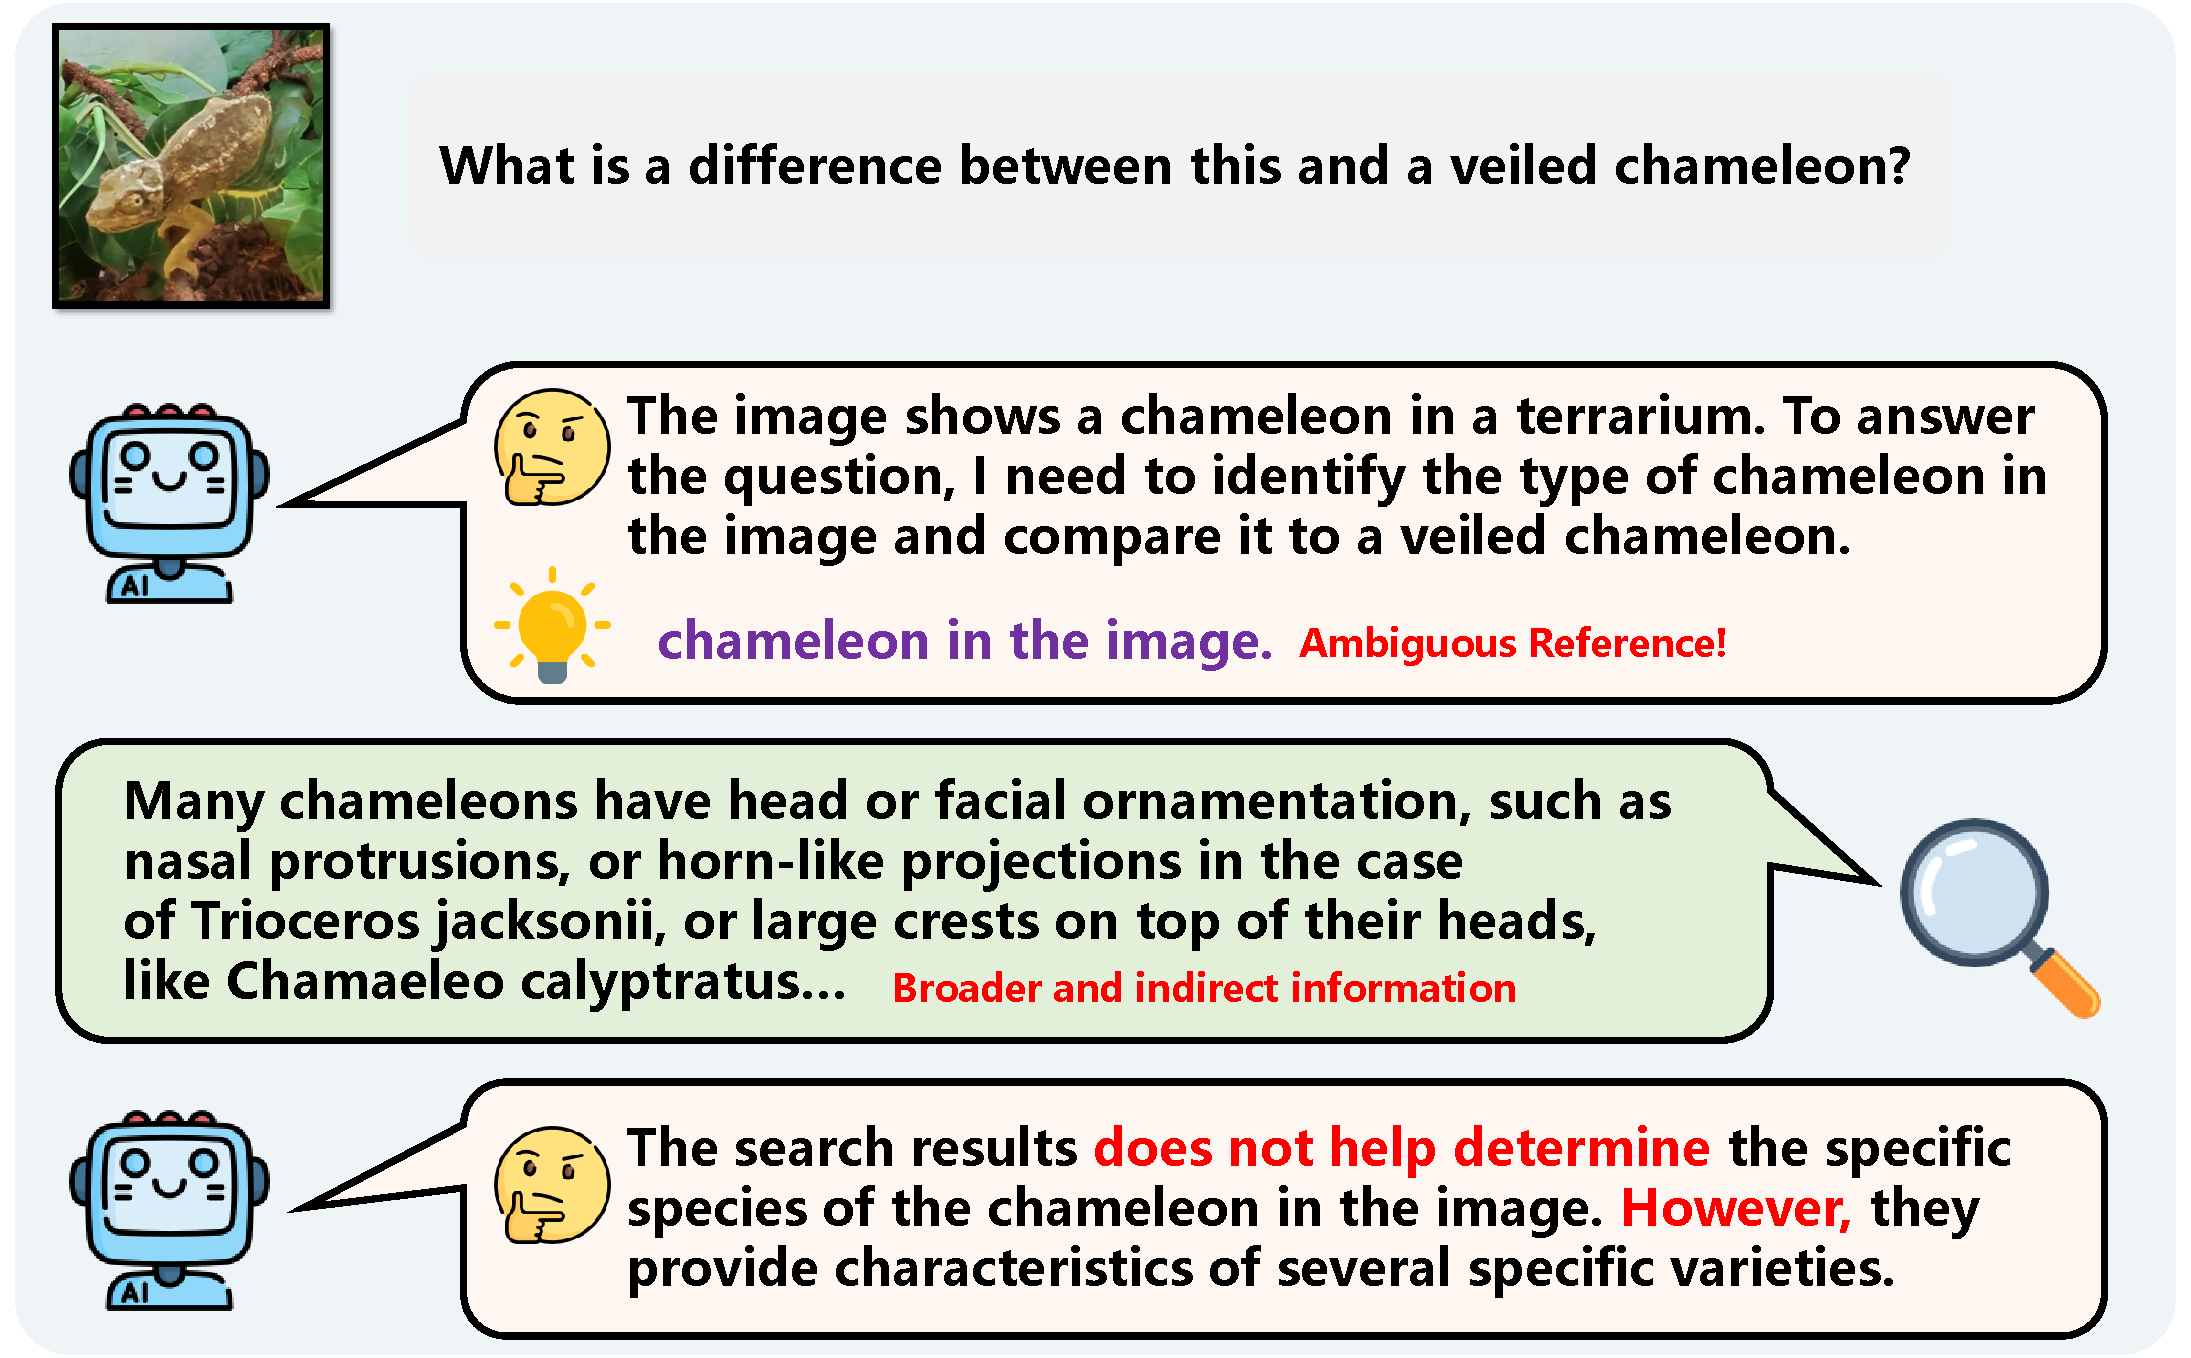
\includegraphics[width=0.5\textwidth]{introduction_1.pdf}
    \caption{The manifestation of vague reference lies in the generalization and general designation of precise entities, making it difficult to accurately locate relevant information about the entities.}
    \label{fig:introduction_phenomenon}
\end{wrapfigure}
Recent advances in retrieval-augmented generation (RAG) have led to the widespread adoption of agentic pipelines, with MM-ReAct~\citep{yang2023mm} being a representative example. This paradigm exhibits the general characteristics of agentic pipelines, including autonomous tool invocation, iterative planning, and feedback-driven adaptation. In VQA, retrievers are often used as tools, and visual language models (VLMs) autonomously determine when to query external knowledge sources, how to formulate sub-questions, and how to plan multi-step reasoning trajectories~\citep{yao2022react,li2024benchmarking}.
While this flexibility enables powerful multi-hop reasoning, it also makes model-generated retrieval queries difficult to control.
The retriever only observes the emitted query string, not the visual context or the latent entity that the VLM intends to ask about.
Consequently, queries that are natural to the VLM may still be under-specified for retrieval~\citep{jin2025search,wu2025mmsearch}: they may emit queries with ambiguous reference such as ``the object in the image'' or ``the person related to it'' without exposing the entity-level anchor required by a text retriever, illustrated in Figure~\ref{fig:introduction_phenomenon}. In this case, both sparse retrieval and dense retrieval can only retrieve more generalized corpus based on surface-level semantics. We refer to this phenomenon as \textbf{Referential Ambiguity}.

From a structural linguistic perspective, following Saussure's classic theory ~\citep{de1916nature}, the relationship between a signifier and its signified is arbitrary and stabilized by context rather than guaranteed by the expression itself.
In agentic multimodal retrieval, each text query is a signifier intended to denote a particular entity in the image or in the external knowledge space.
Referential ambiguity arises when this mapping is unstable: a single query may correspond to multiple plausible entities or fail to uniquely identify the intended referent.
Such ambiguity is especially consequential in agentic pipelines because early retrieval results condition subsequent iterations.

Analysis shows that referential ambiguity is omnipresent in ReAct-style agentic pipelines, especially when visual entity grounding and external knowledge lookup are tightly coupled. Existing work in RAG research often treats ambiguity as a uniformly harmful property of a query, with efforts focused on resolving or refining ambiguity to improve retrieval and downstream generation performance~\citep{chan2024rq,jang2025ambiguity,liu2023we}. In contrast, our controlled interventions show that ambiguity is not a sufficient explanation for trajectory and answer degradation.
The effect of query specificity is structural rather than monotonic: the same rewrite can increase activity on one backbone, leave another largely unchanged, or even suppress a trajectory that would otherwise continue productively.
This suggests that the central issue is not ambiguity itself, but whether the query formulation is compatible with the backbone's latent retrieval policy.

This paper therefore shifts the focus from the conventional question of ``How can referential ambiguity be eliminated?'' toward a more general one: ``When does query clarification help the agent, when does it suppress useful exploration, and what does that reveal about the query--retriever interface?''
We first define referential ambiguity and introduce RefAmb, a multi-source benchmark constructed from CRAG-MM~\citep{yang2024crag}, InfoSeek~\citep{chen2023can}, MC-Search~\citep{ning2026mc}, and OVEN~\citep{hu2023open}, and conduct unified, newly normalized labeling.
We then introduce Retrieval-involved Trajectory Efficiency (RTE) to evaluate the quality of intermediate retrieval-conditioned process dynamics.
Finally, we introduce an auxiliary intervention, \textbf{I}nformation \textbf{I}ncrement \textbf{G}uided \textbf{C}ontext \textbf{R}econstruction (IIGCR), which selectively rebuilds context when the agent enters repeated or uninformative retrieval states.
Experiments show that this intervention can mitigate trajectory decay in the main setting, but it does not remove the backbone dependence of query control.

In short, our contributions are:
\begin{itemize}
    \item We construct \textbf{RefAmb}, a multi-source benchmark for analyzing referential behavior in agentic multimodal retrieval, featuring unified golden-entity annotations and a comprehensive categorization of reasoning structures for VQA tasks.
    \item We develop a \textbf{Trajectory Dynamic Quantification Metric (RTE)}, which evaluates the quality of intermediate processes in the pipeline by scoring the execution dynamics of task-solving steps, thereby enabling a more comprehensive assessment of RAG performance.
    \item Our analysis shows that referential ambiguity is not a universal error signal: its impact on trajectory activity and answer quality depends on backbone family and task structure, revealing a controllability gap at the query--retriever interface.
    \item We observe a recurrent decay of trajectory activity across iterations, but the magnitude and reversibility of that decay are not backbone-invariant, and trajectory efficiency is only partially coupled with final correctness.
    \item We include \textbf{Information Increment Guided Context Reconstruction (IIGCR)} as an auxiliary intervention on low-gain trajectories, showing that context reconstruction can recover some stagnating runs but does not erase the backbone dependence of query control.
\end{itemize}

\section{Curating a VQA-based Multi-source Ambiguity Diagnostic Dataset: RefAmb}
\subsection{Task Taxonomy and Data Composition.}

RefAmb is designed as a \textbf{diagnostic benchmark for referential ambiguity} at the agentic query--retriever interface, rather than a population-level benchmark for natural VQA distributions.
Accordingly, we organize data by \textbf{ambiguity-relevant query structures} that expose where referential under-specification is likely to enter retrieval trajectories.
These task types are \textbf{operational diagnostic bins}, not source-native VQA categories, and their role is to reveal where query-control policies fail to transfer cleanly.

We use five entity-centric task types:
\textbf{Entity Recognition (E.R.)},
\textbf{Single-hop Attribute Query (S.A.Q.)},
\textbf{Multi-hop Reasoning (M.H.)},
\textbf{Comparison (Comp.)},
and \textbf{Compositional Complex Query (C.C.Q.)}.
E.R. emphasizes identifying the target entity itself;
S.A.Q. queries one-hop properties of an identified entity;
M.H. requires chain-style reasoning via intermediate entities/relations;
Comp. requires contrastive reasoning over multiple candidates;
C.C.Q. emphasizes multi-aspect compositional querying centered on a core entity.
This taxonomy is intended to localize ambiguity entry modes in retrieval, rather than to mirror any single dataset's original label system.

To construct these bins while reducing the risk that our observations are artifacts of a single dataset construction, we first collect a multi-source candidate pool from CRAG-MM~\citep{yang2024crag}, InfoSeek~\citep{chen2023can}, MC-Search~\citep{ning2026mc}, and OVEN~\citep{hu2023open}.
Importantly, original dataset tags are treated only as candidate priors.
Final task assignments are produced by a unified post-hoc annotation protocol under the same RefAmb definitions, together with golden-entity grounding and human consistency checks.
Thus, RefAmb task labels are annotation-normalized diagnostic labels rather than direct reuse of source-native taxonomies.

For fair cross-task comparison, we construct a task-balanced analysis subset by stratified sampling without replacement over task type, while preserving the original source mixture within each task. The subset contains a total of 1,500 pieces of data, with 300 pieces for each task type.
Importantly, task-type results in RefAmb should be interpreted as \textbf{source-conditioned diagnostic patterns}, not source-invariant causal effects. The point of the taxonomy is to expose non-uniform regularities in how ambiguity enters the trajectory, not to imply a universal law that holds across every source and backbone. More details on the dataset construction are shown in Figure~\ref{fig:dataset-composition} in Appendix~\ref{app:details_dataset}.

Each item is annotated with four fields: golden entity, \texttt{text\_alone\_identifies\_entity}, \texttt{external\_evidence\_dependency}, and task type.
For InfoSeek, target entities are recovered through OVEN/Wikidata mapping; for OVEN, answer entities are used directly; for CRAG-MM and MC-Search, golden entities are extracted from question--answer context and consistency-checked with GPT-4o.
\subsection{Entity and Ambiguity Annotation}
\begin{wrapfigure}{r}{0.5\textwidth}
    \centering
    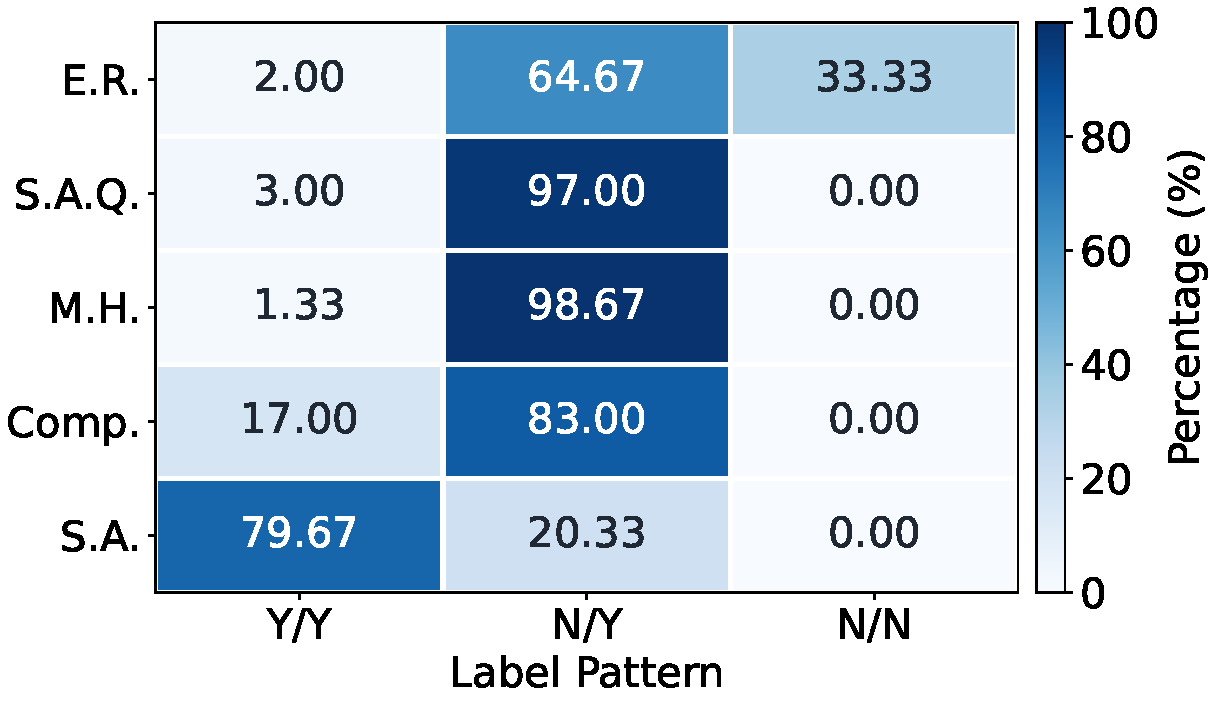
\includegraphics[width=0.5\textwidth]{c1,2_label_2d_by_task_type_heatmap.pdf}

    \caption{Per-task-type distribution on $C_1$ and $C_2$, where each cell is the corresponding labels of $C_1$ and $C_2$.}
    \label{fig:stage1-label-2d-by-task-type}
\end{wrapfigure}
We construct the two diagnostic labels based on the following two questions.
\textbf{$C_1$: Whether the core entity can be identified from the text query alone.}
Given question text $q$ and golden entity $\gold$, we assign
\texttt{text\_alone\_identifies\_entity=Yes} iff $q$ already contains enough lexical evidence to identify $\gold$ without looking at the image.
Operationally, this is anchored by explicit entity mention and alias-level matching against the golden entity list; otherwise the label is \texttt{No}. This indicator reflects the modal coupling of the query.
\textbf{$C_2$: Whether external knowledge is essential to answer the text query.}
We use a semi-manual and semi-large-model two-stage protocol to reduce contamination from model parametric memory.
The first stage extracts explicit visual clues from the image that are relevant to the question.
The next stage judges whether the final answer can be \textbf{directly supported by only} these explicit clues plus the question text, without invoking world knowledge.
If the answer is not supportable under this constraint, we assign \texttt{external\_evidence\_dependency=Yes}; otherwise \texttt{No}.
This separates evidence sufficiency from ``the model happens to know the fact''.
As shown in Figure~\ref{fig:stage1-label-2d-by-task-type},
Entity Recognition is the most image-coupled family, so the query often cannot stand on its own and the image is doing most of the work in resolving both $C_1$ and $C_2$.
Single-hop Attribute Query and Multi-hop are different in form but similar in mechanism: they ask for attributes, relations, or derived facts that are not fully encoded in the surface wording, so the text often leaves the entity underdetermined while the answer still depends on outside knowledge.
Comparison tasks are structurally mixed, because one side of the comparison may already be explicit while the other still needs to be inferred; that is why both $C_1$ outcomes naturally coexist there.
Subproblem Aggregation is driven by chained decomposition around a core entity, and in MCSearch the image usually acts as supporting context rather than the primary identifier, so the table reflects a much stronger reliance on text-side entity anchoring than on visual disambiguation alone.

% \begin{table}[t]
% \centering
% \begin{threeparttable}
% \small
% \caption{Per-task-type distribution on $C_1$ and $C_2$, where each cell is the corresponding labels of $C_1$ and $C_2$.}
% \begin{tabular}{lrrr}
% \hline
% \textbf{Task Type} & \textbf{Yes/Yes} & \textbf{No/Yes} & \textbf{No/No}\\
% \hline
% Entity Recognition & 2.00\% & 64.67\% & 33.33\% \\
% Single-hop Attribute Query & 3.00\% & 97.00\% & 0.00\% \\
% Multi-hop & 1.33\% & 98.67\% & 0.00\% \\
% Comparison & 17.00\% & 83.00\% & 0.00\% \\
% Subproblem Aggregation & 79.67\% & 20.33\% & 0.00\% \\
% \hline
% \end{tabular}
% \label{tab:stage1-label-2d-by-task-type}
% \end{threeparttable}
% \end{table}

% \begin{figure}[htbp]
%     \centering
%     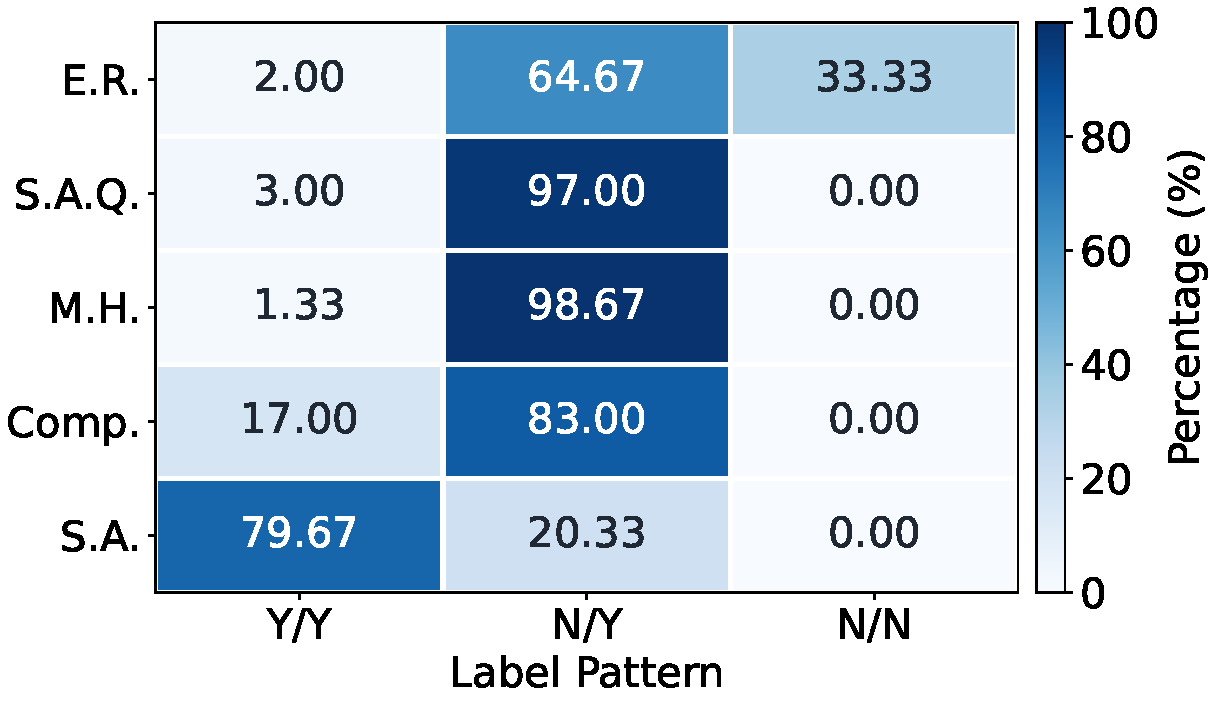
\includegraphics[width=0.8\linewidth]{c1,2_label_2d_by_task_type_heatmap.pdf}
%     \caption{Per-task-type distribution on $C_1$ and $C_2$, where each cell is the corresponding labels of $C_1$ and $C_2$.}
%     \label{fig:stage1-label-2d-by-task-type}
% \end{figure}


\subsection{Retrieval-involved Trajectory Efficiency}
Endpoint metrics such as exact match, F1, or GPT-based answer accuracy do not directly explain how a trajectory evolves. 
We therefore propose a metric suite for quantifying retrieval-involved trajectory efficiency, including factual information increment $\Delta F$, which captures whether a retrieval step introduces new facts, retrieval utility $U_t$, which assesses whether the agent's subsequent thought effectively exploits the retrieved evidence, and ultimately Retrieval-involved Trajectory Efficiency (RTE), which summarizes the overall quality of retrieval-conditioned trajectory evolution.
\paragraph{Retrieval-step notation.}
Let $\mathcal{T}=\{1,\ldots,T\}$ denote the index set of ordered text-retrieval steps extracted from a full ReAct trajectory.
For each text-retrieval step $t\in\mathcal{T}$, $\query_t$ is the emitted text query and $r_t$ is the retrieved textual evidence.
We extract from $r_t$ a set of atomic factual units $\facts_t=\{f_{t,1},\ldots,f_{t,n_t}\}$.
The accumulated fact history before step $t$ is denoted as $\facts_{<t}$, and the updated history is
\begin{equation}
    \facts_{\leq t} = \facts_{<t} \cup \facts_t.
\end{equation}
In implementation, both within-step and cross-step fact unions are deduplicated by semantic similarity so that near-duplicate retrieved statements are not counted as new evidence.

\paragraph{Query-similarity gate.}
Before measuring factual novelty, we first check whether the current text query simply repeats the previous text query.
We define a query-similarity operator
\begin{equation}
    \operatorname{sim}(\query_t,\query_{t-1})
    =
    \frac{
    \phi(\query_t)^\top \phi(\query_{t-1})
    }{
    \|\phi(\query_t)\|_2 \, \|\phi(\query_{t-1})\|_2
    },
\end{equation}
The binary repetition gate is then
\begin{equation}
    G_t = \mathbf{1}\!\left[\operatorname{sim}(\query_t,\query_{t-1}) < 1\right].
\end{equation}
Thus $G_t=0$ only for exact repeated queries under the similarity implementation, while non-identical queries are still evaluated by their retrieved factual novelty.

\paragraph{Factual Novelty.}
The raw factual increment counts the proportion of retrieved facts at step $t$ that are absent from the previous fact history, named as \textbf{New-Fact Ratio}:
\begin{equation}
    \Delta F_t^{\mathrm{raw}}
    =
    \frac{|\facts_{\leq t} \setminus \facts_{<t}|}{|\facts_t|+\epsilon}.
\end{equation}
Equivalently, using the union update above,
\begin{equation}
    \Delta F_t^{\mathrm{raw}}
    =
    \frac{|\facts_t \cup \facts_{<t}| - |\facts_{<t}|}{|\facts_t|+\epsilon}.
    \label{eq:delta_f}
\end{equation}
Here $\epsilon\rightarrow0^+$ is a small constant for numerical stability when no valid factual unit is extracted.
The final factual novelty combines the repetition gate and raw factual novelty:
\begin{equation}
    \df_t = G_t \cdot \Delta F_t^{\mathrm{raw}}.
    \label{eq:delta_f_whole}
\end{equation}
This decomposition separates two failure modes: repeated querying is captured by $G_t$, while non-repeated but uninformative retrieval is captured by a low $\Delta F_t^{\mathrm{raw}}$.

\paragraph{Iteration Utility.}
Factual novelty alone does not show whether the agent can use the newly retrieved evidence.
For each retrieval step, we inspect the following \texttt{<Thought>} block, which is conditioned on the retrieval result from the preceding step.
This post-retrieval thought provides a trajectory-internal signal of whether the agent treats the evidence as irrelevant, partially helpful, or sufficient.
We map these labels to an ordinal utility variable
\begin{equation}
    U_t \in \{0,\;0.5,\;1\},
    \label{eq:u_t}
\end{equation}
where $0$ means no contribution, $0.5$ means partial contribution, and $1$ means full contribution.
The midpoint is used as an interpretable ordinal weight, not as a claim that utility is interval-scaled.

\paragraph{Final RTE score.}
The retrieval-conditioned contribution of step $t$ is
\begin{equation}
    S_t = U_t \cdot \df_t.
    \label{eq:s_t}
\end{equation}
The trajectory-level score is the average over text-retrieval steps:
\begin{equation}
    \rte(\tau) = \frac{1}{|\mathcal{T}|}\sum_{t\in\mathcal{T}} S_t.
    \label{eq:rte}
\end{equation}
A high RTE therefore requires both factual novelty and reasoning utility.
Repeated searches, empty retrieval, redundant evidence, and evidence that the model ignores all receive low scores.
Thus RTE is not merely a syntactic trajectory statistic; it captures process quality that is related to final generation quality.

\section{Mechanism Analysis of Referential Ambiguity on RefAmb}


\subsection{Setup}
We evaluate a MM-ReAct pipeline using Qwen2.5-VL-7B-Instruct as the main backbone based on the FlashRAG toolkit~\citep{jin2025flashrag}. The core implementation follows OmniSearch~\citep{li2024benchmarking}, but we reengineered it to improve robustness. More details are shown in Appendix~\ref{app:experiment_setup_details}.

We examine three experimental conditions.
\textbf{Original} corresponds to the unmodified agent trajectories.
\textbf{Oracle Intervention} implements a static-context reconstruction and targeted query rewriting mechanism. Based on the recorded trajectories under the Original setting, trajectories are first classified according to the occurrence of referential ambiguity. For trajectories exhibiting ambiguity, the first retrieval query identified as entity-ambiguous is replaced with its annotated canonical entity. The rewritten query is then used to perform retrieval, and the resulting evidence replaces the original retrieved content, with the previous model feedback removed. Subsequently, the trajectory preceding the first ambiguous step is reconstructed and fed back into the backbone model, allowing it to continue iterative reasoning without additional intervention.

\textbf{Disturb Intervention} follows an analogous procedure, but is applied to originally unambiguous first-round queries: the central entity in the query is deliberately transformed into a generalized or referential expression. The modified query is used to retrieve new evidence, which replaces the original retrieval, and the trajectory preceding the first perturbed step is reconstructed for continuation by the model.
All interventions are confined to query formulation; the agent continues its reasoning process from the modified retrieval evidence, allowing us to isolate the effects of controlled ambiguity and canonical entity alignment on trajectory efficiency and final answer quality.
The detection of all entity-ambiguous queries and query rewriting are performed by GPT-4o; fact extraction in RTE values is conducted by Qwen2.5-7B, and utility evaluation is carried out by GPT-4o. The appendix records the consistency between their evaluation results and human annotations.

% \begin{table}[htbp]
% \centering
% \begin{threeparttable}
% \small
% \caption{Referential ambiguity frequency in RefAmb by task type. Ambiguity is frequent overall, but its prevalence varies sharply with task structure and referential dependence.}
% \begin{tabular}{llrrr}
% \toprule
% \textbf{Task Type} & \textbf{Scale} & \textbf{Total} & \textbf{Ambiguous} & \textbf{Frequency} \\
% \midrule
% \multirow{2}{*}{Overall}  & Item scale  & 1500 & 460  & 30.67\% \\
%                            & Query scale & 4433 & 1412 & 31.85\% \\
% \multirow{2}{*}{Entity Recognition}          & Item scale  & 300  & 79  & 26.33\% \\
%                                               & Query scale & 534  & 235 & 44.01\% \\
% \multirow{2}{*}{Single-hop Attribute Query}   & Item scale  & 300  & 141 & 47.00\% \\
%                                               & Query scale & 999  & 474 & 47.45\% \\
% \multirow{2}{*}{Multi-hop}                    & Item scale  & 300  & 125 & 41.67\% \\
%                                               & Query scale & 1070 & 361 & 33.74\% \\
% \multirow{2}{*}{Comparison}                   & Item scale  & 300  & 99  & 33.00\% \\
%                                               & Query scale & 1031 & 313 & 30.36\% \\
% \multirow{2}{*}{Subproblem Aggregation}       & Item scale  & 300  & 16  & 5.33\% \\
%                                               & Query scale & 799  & 29  & 3.63\% \\
% \bottomrule
% \end{tabular}
% \label{tab:ambiguity-frequency}
% \end{threeparttable}
% \end{table}

It can be observed from Table~\ref{tab:ambiguity_frequency_source} that the occurrence frequency of referential ambiguity is neither rare nor universal: it changes substantially across model families, source distributions, and task structures.
In particular, the Qwen3 family shows a wide spread across scales, while InternVL3.5-8B and Qwen2.5-VL-7B remain much more ambiguity-prone than the smaller or better-aligned backbones.
This variability suggests that ambiguity is not simply a property of the dataset, but also a property of the backbone's query-generation policy.
\subsection{Controlled Ambiguity Reveals Structural Dynamics in Agentic Retrieval Trajectories}
\begin{figure}[htbp]
    \centering
    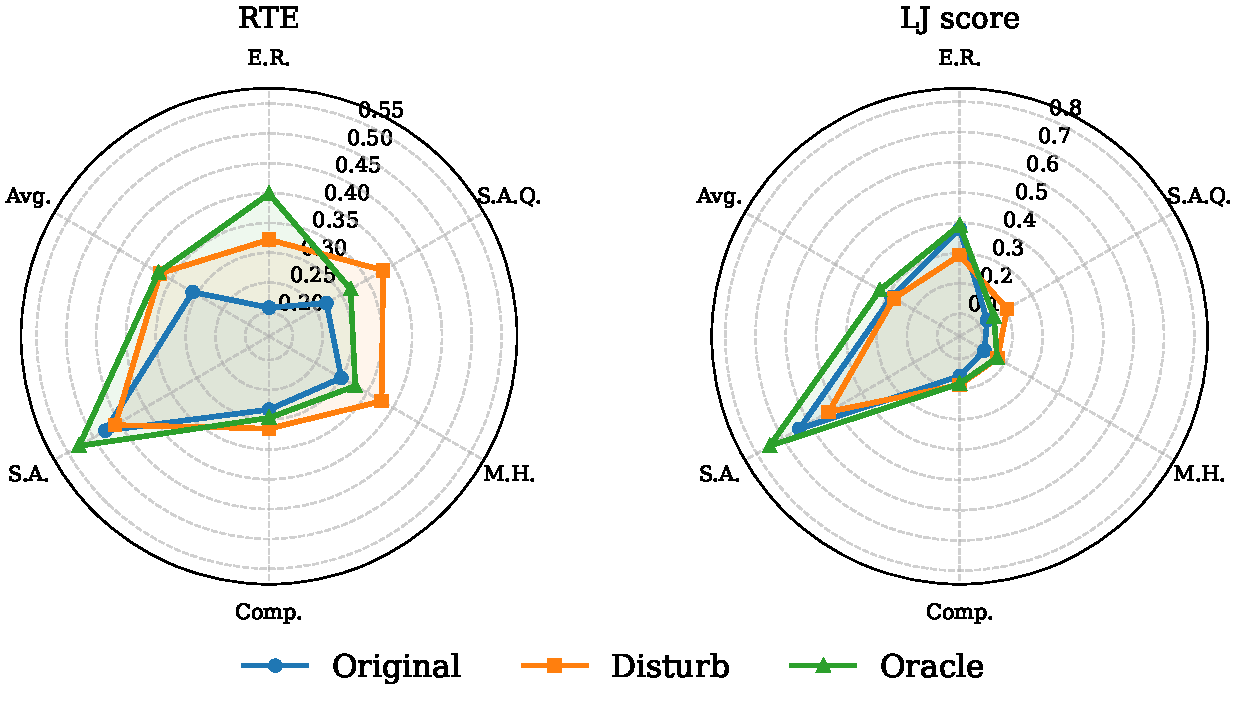
\includegraphics[width=0.7\linewidth]{trajectory_quality_overall.pdf}
    \caption{Trajectory activity (RTE) and final generation quality (LLM-as-Judge) under the two intervention settings.}
    \label{fig:trajectory_quality_overall}
\end{figure}
We calculate the average values of RTE and LJ for samples of each task category under every setting. The former is used to measure the activity of trajectories, namely whether effective information retrieval is being conducted continuously, while the latter is adopted to evaluate the correctness of the generation results produced by the pipeline itself. To further control the inherent bias of samples, we classify samples not only by task category but also according to whether the pipeline gives correct answers. We then compare Oracle, Original, and Disturb on samples with correct and incorrect responses respectively.

\paragraph{Disturb Intervention} 
As illustrated in Figure~\ref{fig:trajectory_quality_overall}, Disturb can raise trajectory activity on the main Qwen2.5 setting, and in a few subtasks it also improves the final answer signal relative to the original pipeline.
This makes the intervention useful as a probe of exploratory relaxation: deliberate ambiguity can broaden the retrieval neighborhood and temporarily increase the amount of novel evidence entering the trajectory.
However, the same figure also shows that increased activity does not reliably translate into better final answers, especially outside the entity-centric regime.
The cross-model validation later in this section makes the boundary clearer: the exploration boost visible on Qwen2.5 does not transfer uniformly to InternVL3.5 or the Qwen3 family, where Disturb often reduces trajectory quality instead of improving it.
We therefore interpret Disturb as evidence that ambiguity can sometimes stimulate exploration, but only within a backbone-specific operating region.
\begin{figure}
    \centering
    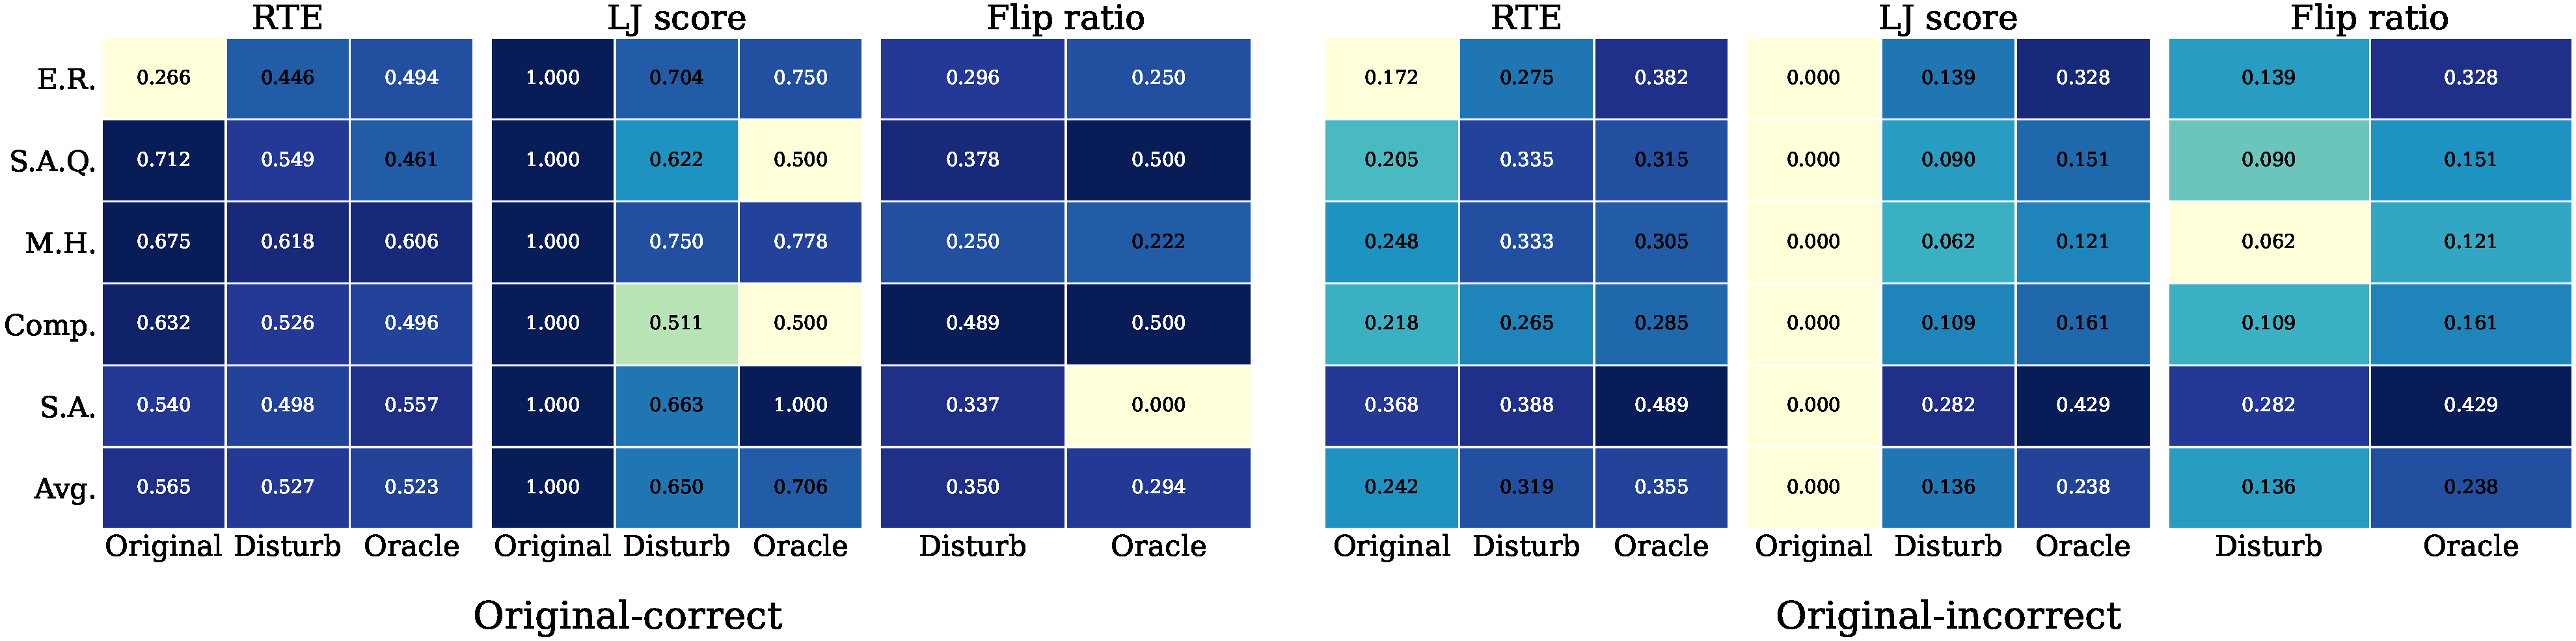
\includegraphics[width=\linewidth]{trajectory_quality_main_heatmap.pdf}
    \caption{Trajectory samples under the correctness category, comparing RTE, LJ, and answer-correctness flip rate between the two intervention settings and the baseline. The flip ratio is the rate at which originally correct (incorrect) answers are turned into incorrect (correct) ones.}
    \label{fig:trajectory_quality_main_heatmap}
\end{figure}

Furthermore, the heatmaps in Figure~\ref{fig:trajectory_quality_main_heatmap} reveal the asymmetric effects of Disturb and Oracle interventions on trajectory dynamics.
For samples where the Original pipeline already produces correct answers, both interventions typically reduce average trajectory efficiency and final answer fidelity.
The decline in RTE is often smaller under Disturb, whereas Oracle more directly suppresses answer-level flips in the main Qwen2.5 setting.
Conversely, for samples initially answered incorrectly, both interventions can improve the trajectory signal, with Oracle usually providing the more reliable repair in the Qwen2.5 backbone.
Taken together, these results show that query rewriting changes the balance between exploration and grounding, but the conversion of that change into final correctness is unstable and depends on the backbone and task regime.
\paragraph{Oracle Intervention} 
Analysis of trajectory and generative metrics within the diagnostic regimes of RefAmb shows that Oracle intervention is the most stable repair strategy on Qwen2.5-VL-7B, especially for entity-centric samples.
Precise entity grounding provides a cleaner retrieval signal and often improves both trajectory dynamics and final answer fidelity when the backbone is already compatible with the rewrite.
Yet the cross-model validation later in the paper shows that this benefit is not backbone-invariant: on several Qwen3 variants, the same canonical rewrite reduces RTE or leaves it unchanged even when it removes ambiguity.
We therefore interpret Oracle as a targeted repair mechanism rather than a universally beneficial intervention.

Analysis of the VLM trajectories under Oracle interventions, stratified by Original correctness, reveals a nuanced interplay between retrieval augmentation and the model’s internal inferential apparatus.
For the Original-correct subset, both final answer fidelity and trajectory dynamics can decrease relative to the Original pipeline, which means that even precise ground-truth entity information is not automatically beneficial.
This is consistent with the idea that a rewrite may remove ambiguity while also suppressing a useful exploratory path.
Conversely, for the Original-incorrect subset, Oracle often enhances both trajectory and generative metrics, demonstrating that precise entity grounding can remediate previously failed trajectories when the backbone already accepts the rewritten control signal.

Referential ambiguity therefore does not fit a simplistic dichotomy in which ambiguity is harmful and precision is always beneficial.
Precise entity grounding is often the safer default, but it can still perturb a trajectory that was already using a productive exploration policy.
Controlled ambiguity can stimulate exploratory capacity, but the resulting gain is backbone-dependent and does not transfer uniformly across task types or model families.

\subsection{Inhibition Effect of Two Types of Interventions on Pipeline Inactivation}
As stated above, Disturb can improve trajectory activity in the main Qwen2.5 setting, but this activity does not automatically convert into higher-quality answers.
Oracle achieves cleaner recovery on the main backbone, yet the activity gain is still far from ideal and remains conditional on the backbone accepting the rewrite.
To further analyze the reasons, we next inspect repeated queries and zero-information steps.
As shown in Table~\ref{tab:refamb-stagnation-ratios}, a substantial fraction of steps in original trajectories exhibits zero-information or exact repeated queries, reflecting pronounced stagnation.
Disturb alleviates this most strongly in the Qwen2.5 setting, reducing both repeated-query and zero-$\Delta F$ rates relative to original, whereas Oracle achieves a moderate reduction.
Mean $\Delta F$ per step increases under both interventions in Qwen2.5, which is consistent with the idea that controlled ambiguity can stimulate exploration and reduce stagnation locally.
\begin{table}[htbp]
\centering
\begin{minipage}[c]{0.48\textwidth}
  \centering
  \captionof{table}{The overall ratio of repeated queries and zero-information steps.}
  \begin{tabular}{lcc}
    \hline
    \textbf{Setting} & \textbf{Repetitious Queries} & \textbf{$\Delta F=0$} \\
    \hline
    Original & 34.6\% & 46.0\% \\
    Oracle & 28.5\% & 36.0\% \\
    Disturb & 25.4\% & 35.3\% \\
    \hline
  \end{tabular}
  \label{tab:refamb-stagnation-ratios}
\end{minipage}
\hfill
\begin{minipage}[c]{0.48\textwidth}
  \centering
  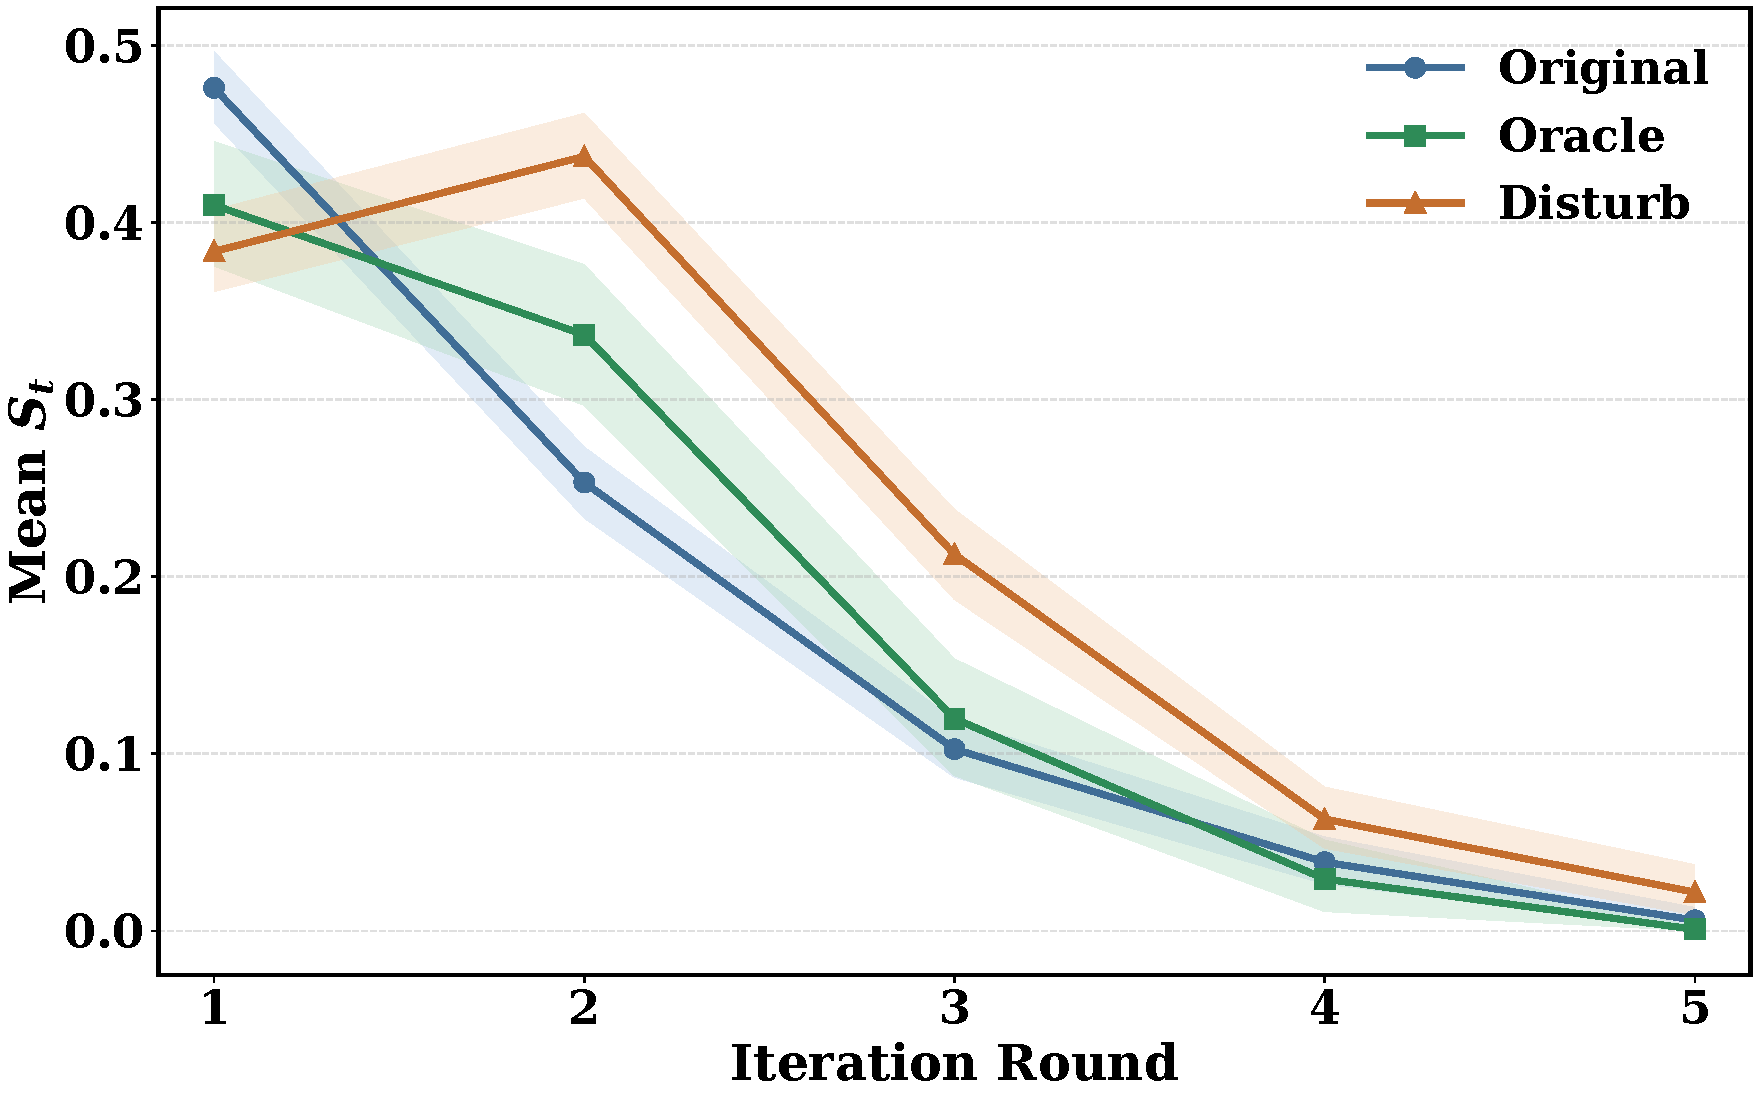
\includegraphics[width=\linewidth]{refamb_step_score_curve.pdf}
  \captionof{figure}{Mean step score $S_t$ by retrieval iteration.}
  \label{fig:stagnation-curve}
\end{minipage}
\end{table}
Figure~\ref{fig:stagnation-curve} shows that at the initial steps, the step-level contribution $S_t$ does not differ substantially across the three settings.
Disturb initially causes a small decrease in $S_t$, but as iterations progress, it can elevate the trajectory's activity in the Qwen2.5 setting, keeping it above both Original and Oracle in later rounds.
Oracle also raises trajectory activity slightly, although the effect is smaller.
Importantly, the decline in $S_t = U_t \cdot \Delta F_t$ is not unique to any single intervention: all three settings show a broadly monotone decrease in marginal factual gain, and the trajectories nearly collapse in the final rounds.
We refer to this late-iteration flattening and convergence across settings as \textbf{Trajectory Stagnation}, which is primarily manifested through repeated query generation.
The key point is not that interventions remove stagnation, but that they shift the operating point of the trajectory by different amounts, with the size of that shift depending on the backbone.
\subsection{Cross-Model Transfer of Intervention Effects}
The new cross-model intervention results sharpen the boundary of this effect.
On Qwen2.5-VL-7B, Oracle and Disturb can raise the mean trajectory score and, for some tasks, improve final correctness, which is consistent with the main-body analysis above.
InternVL3.5-8B still shows a useful Oracle gain, but the margin is smaller and the Disturb setting is already less favorable, indicating that the repair signal is weaker outside the main backbone.
By contrast, the Qwen3 family is much less forgiving: both Disturb and Oracle usually reduce trajectory quality relative to Original, with only Entity Recognition retaining a clear positive Oracle effect.
This pattern is important because it rules out a backbone-invariant reading of the intervention results.
The same rewrite policy can remove ambiguity while still lowering RTE, which means that canonicalization is not a universal improvement but a backbone-dependent control operation.
Accordingly, the main discovery is not that ambiguity is always helpful or always harmful.
The stronger claim is that query-specific control has a controllability gap across backbones: some models translate canonical grounding into better trajectories, while others do not.
\section{Auxiliary Intervention for Trajectory Decay}
Based on the conclusion mentioned above, trajectory dynamics decay as the iteration count grows, but the effect of query rewriting is not invariant across backbones.
This means that large-model calls do not necessarily convert into proportional gains unless the rewrite aligns with the backbone's latent retrieval policy.
To probe whether low-gain trajectories can be partially recovered, we introduce an auxiliary intervention, \textbf{I}nformation \textbf{I}ncrement \textbf{G}uided \textbf{C}ontext \textbf{R}econstruction (abbreviated as IIGCR).
The overall framework is shown in Figure~\ref{fig:method_overview}, and the detailed algorithm is given in Appendix~\ref{app:algorithm}.
\begin{figure}[htbp]
    \centering
    
\includegraphics[width=\linewidth]{method_overview.pdf}
    \caption{Auxiliary intervention based on IIGCR for low-gain trajectories.}
    \label{fig:method_overview}
\end{figure}

\paragraph{Information Guided Rewrite Logics}
Based on detailed case analyses, we posit that repeated queries emerge primarily when the VLM treats the current retrieved corpus as insufficient to resolve the active sub-problem.
This observation motivates a principled approach to trajectory-blocking prediction.
Concretely, we operationalize query rewriting through two modes, \texttt{missing\_info} and \texttt{reflection}, governed by two explicit gating mechanisms.
For query repetition, let $q_t$ denote the current query and $q_{t-1}$ the preceding one; a repair is triggered when $\mathrm{sim}(q_t,q_{t-1}) > \tau_s$, with $\mathrm{sim}(\cdot)$ defined as cosine similarity.
For low-yield retrieval, the repair is initiated when $\Delta F_t < \tau_f$, where $\Delta F_t$ represents the step-level information increment ratio used in RTE.
Under either gating condition, \texttt{missing\_info} directs the subsequent \texttt{<Search>} action toward a distinct missing clue spanning entity, attribute, relation, temporal, or spatial facets, and incorporates a correctness verification mechanism.
If this mode of rebuilding repeats and still fails, the rewrite process switches to \texttt{reflection} mode, enforcing a more substantial rollback of recent low-gain steps and mandating a reoriented retrieval strategy.
Verified formatted actions replace the original query in a minimally intrusive manner. Detailed algorithms are provided in Appendix~\ref{app:algorithm}.
\paragraph{Pruning Based Context Intervention}
Messages rebuilt under \texttt{reflection} mode are injected as revised Search actions, and the dialogue trajectory is pruned and rebuilt accordingly.
As the context-pruning module in Figure~\ref{fig:method_overview} illustrates, instead of only replacing a \texttt{<Search></Search>} span, we remove low-contribution or duplicated retrieval states along with their adjacent feedback segments from back to front until all inefficient iterations are eliminated, then continue inference with a cleaner context.
When low-$\Delta F$ behavior persists, this pruning improves context utility and stabilizes subsequent reasoning.
\subsection{Main Results} 
\begin{table}[htbp]
\centering
\small
\setlength{\tabcolsep}{3pt}
\caption{Main baselines grouped by inference style across task types.}
\resizebox{\linewidth}{!}{%
\begin{tabular}{l|cc|cc|cc|cc|cc|cc}
\toprule
\multirow{2}{*}{\textbf{Method}} & \multicolumn{2}{c|}{\textbf{EntityRecognition}} & \multicolumn{2}{c|}{\textbf{SinglehopAttributeQuery}} & \multicolumn{2}{c|}{\textbf{Multihop}} & \multicolumn{2}{c|}{\textbf{Comparison}} & \multicolumn{2}{c|}{\textbf{SubproblemAggregation}} & \multicolumn{2}{c}{\textbf{Overall}} \\
\cmidrule(lr){2-3}
\cmidrule(lr){4-5}
\cmidrule(lr){6-7}
\cmidrule(lr){8-9}
\cmidrule(lr){10-11}
\cmidrule(lr){12-13}
 & \textbf{RTE} & \textbf{LJ} & \textbf{RTE} & \textbf{LJ} & \textbf{RTE} & \textbf{LJ} & \textbf{RTE} & \textbf{LJ} & \textbf{RTE} & \textbf{LJ} & \textbf{RTE} & \textbf{LJ} \\
\midrule
\multicolumn{13}{c}{\textit{\textbf{ReAct-style RAG}}} \\
\midrule
Qwen2.5-VL-7B & 0.21 & 0.38 & 0.27 & 0.13 & 0.30 & 0.12 & 0.28 & 0.16 & 0.48 & 0.64 & 0.31 & 0.28 \\
InternVL3.5 & 0.13 & 0.27 & 0.08 & 0.03 & 0.03 & 0.01 & 0.02 & 0.00 & 0.46 & 0.33 & 0.14 & 0.13 \\
Qwen3-VL-32B-Instruct & -- & -- & -- & -- & -- & -- & -- & -- & -- & -- & -- & -- \\
\midrule
\multicolumn{13}{c}{\textit{\textbf{Prompt Optimization of ReAct}}} \\
\midrule
Qwen2.5-VL-7B & -- & -- & -- & -- & -- & -- & -- & -- & -- & -- & -- & -- \\
\midrule
\multicolumn{13}{c}{\textit{\textbf{Ambiguity / Retrieval Control Baselines}}} \\
\midrule
Self-Ask + Search & -- & -- & -- & -- & -- & -- & -- & -- & -- & -- & -- & -- \\
FLARE & -- & -- & -- & -- & -- & -- & -- & -- & -- & -- & -- & -- \\
AmbigPrompt & -- & -- & -- & -- & -- & -- & -- & -- & -- & -- & -- & -- \\
DWE & -- & -- & -- & -- & -- & -- & -- & -- & -- & -- & -- & -- \\
AMELI & -- & -- & -- & -- & -- & -- & -- & -- & -- & -- & -- & -- \\
\textbf{ATL-CI} & \textcolor{red}{0.29} & \textcolor{red}{0.47} & \textcolor{red}{0.40} & \underline{0.21} & \underline{0.42} & \underline{0.19} & \textcolor{red}{0.38} & \textcolor{red}{0.27} & \underline{0.53} & 0.65 & \textcolor{red}{0.41} & \underline{0.36} \\
\quad -w/o Entity Tightening & \underline{0.28} & 0.44 & \underline{0.37} & \underline{0.21} & \textcolor{red}{0.43} & \textcolor{red}{0.20} & \textcolor{red}{0.38} & \textcolor{red}{0.27} & \textcolor{red}{0.54} & \textcolor{red}{0.69} & \underline{0.40} & \textcolor{red}{0.36} \\
\quad -w/o Exploration Activity & 0.26 & \underline{0.46} & 0.36 & 0.19 & 0.38 & 0.17 & 0.33 & 0.21 & 0.51 & \underline{0.67} & 0.37 & 0.34 \\
\quad -w/o ROI & \textcolor{red}{0.29} & 0.43 & \textcolor{red}{0.40} & \textcolor{red}{0.23} & \underline{0.42} & 0.19 & \underline{0.37} & \underline{0.25} & \underline{0.53} & 0.66 & \underline{0.40} & 0.35 \\
\bottomrule
\end{tabular}%
}
\label{tab:main-baselines-tasktype-rte-lj}
\end{table}




\section{Conclusion}
We studied referential ambiguity in agentic multimodal retrieval through RefAmb, RTE, and controlled Original/Oracle/Disturb interventions.
The data do not support a simplistic claim that ambiguity always harms retrieval trajectories, but they also do not support the opposite claim that ambiguity is inherently helpful.
Instead, the strongest result is a controllability gap: the same query rewrite can improve, preserve, or degrade a trajectory depending on the backbone and task regime.
Oracle-style canonical grounding is the most reliable repair on entity-centric trajectories, yet its benefit does not transfer uniformly to newer Qwen3 backbones.
Our analysis therefore suggests a sharper conclusion than the usual ambiguity-versus-precision framing: query specificity should be treated as a backbone-dependent control variable, not as a universal quality signal, and agentic retrieval methods should be evaluated by how well their control policy transfers across backbones.
The auxiliary IIGCR intervention shows that some trajectory decay can be partially mitigated once it is detected, but it is not the main contribution of the paper.

\clearpage
\bibliography{iclr2026_conference}
\bibliographystyle{iclr2026_conference}
\clearpage
\appendix
\onecolumn
\textbf{\Large Appendix}

\addcontentsline{toc}{section}{Appendix}

\startcontents[appendix]

\vspace{1em}
\section*{Contents}
\printcontents[appendix]{}{1}{}

\clearpage
% \section{Appendix}
\section{Related Work}
\subsection{Visual Question Answering}
Visual Question Answering (VQA) was formally introduced by ~\citep{antol2015vqa}, to evaluate whether models can answer natural-language questions grounded in visual inputs. 
Given an image and a question referring to its visual content, a VQA system is expected to infer the relevant visual semantics and return a correct answer. 
Over time, VQA has expanded beyond early single-image, classification-style benchmarks to encompass compositional reasoning, external knowledge acquisition, and instruction-following scenarios~\citep{antol2015vqa, hudson2019gqa}.
Classical VQA datasets mainly emphasize perceptual recognition and short-answer supervision, while newer datasets stress long-tail entities, multi-hop reasoning, and external-knowledge dependence ~\citep{marino2019ok, schwenk2022okvqa}. 

Methodologically, the field has progressed through several stages. 
Early systems predominantly followed CNN--RNN style answer classification pipelines, which were effective for simple recognition but weak at fine-grained grounding and compositional reasoning ~\citep{kazemi2017show}. 
Attention and multimodal fusion methods then improved region--question alignment, yet still relied heavily on static parametric memory ~\citep{lu2016hierarchical}. 
Large-scale pretraining and transformer-based LVLMs further improved generalization and reasoning breadth, but exposed persistent issues in factual reliability and knowledge freshness ~\citep{chen2019uniter}. 
To address these limits, VQA has increasingly moved toward retrieval-augmented paradigms that ground generation in external evidence, and more recently toward agentic workflows with iterative planning, query refinement, and tool-assisted retrieval control ~\citep{abootorabi2025ask,mei2025survey}.

% Despite strong progress in end-to-end answer quality, most VQA evaluations remain endpoint-centric and under-specify how retrieval queries are formed and revised during iterative reasoning ~\citep{vqa_eval_placeholder}. 
% Our work is complementary: instead of treating retrieval as a black box, we analyze query-level referential behavior, ambiguity-triggered control dynamics, and trajectory vitality in retrieval-involved multimodal QA.

\subsection{Agentic Retrieval Augmented Generation}
Agentic RAG extends retrieve-then-read pipelines by letting the model plan sub-queries, trigger retrieval, and invoke tools inside a trajectory-conditioned loop. In visual retrieval more broadly, systems such as ~\citep{yu2025visrag,sun2025visrag} focus on vision-native retrieval and indexing rather than agentic planning. By contrast, agentic multimodal methods such as MM-ReAct based pipeline~\citep{yang2023mm}, ~\citep{li2024benchmarking}, planning agent like CogPlanner~\citep{yu2025cogplanner}, multi-agent paradigm like ViDoRAG~\citep{wang2025vidorag}, and HEAR~\citep{chen2025hear} move toward iterative planning and retrieval control, while ~\citep{zhang2024mr} and ~\citep{qi2024rora} further explore retrieval-reflection and robustness under complex visual evidence.

Compared with these methods, our focus is narrower: we study the impact of ambiguously referring entity queries in VLM-driven retrieval pipelines, where the model must call retrieval tools and generate queries on its own, and analyze how such queries affect trajectory efficiency and generation quality. This is a diagnostic and mechanistic study whose findings motivate an auxiliary intervention for low-gain trajectories.

\subsection{Entity Grounding and Co-reference}
Coreference resolution studies how to link mentions that refer to the same entity. Representative neural approaches include end-to-end antecedent scoring \citep{lee2017end}, joint mention detection and clustering \citep{zhang2018neural}, span pretraining \citep{joshi2020spanbert}, and query-based span prediction \citep{wu2020corefqa}.

In multimodal settings, the task becomes visual reference resolution or multimodal coreference. \citep{kang2019dual} resolves ambiguous questions by combining dialog history with image grounding, while \citep{guo2022gravl} and \citep{inadumi2025disambiguating} model reference over visual and textual context in visually grounded dialogue.

These works assume the ambiguous mention is already given and focus on resolving it from context. Our setting is different: the model must first generate the retrieval query inside an agentic pipeline, so the ambiguity is introduced before retrieval and propagates through the whole trajectory. We therefore study how vaguely referring entity queries affect trajectory efficiency and generation quality, and use that diagnosis to motivate an auxiliary exploration-oriented intervention.
\section{Problem Formulation}
\subsection{Agentic Multimodal Retrieval}
Given an image $I$ and a question $x$, an agentic multimodal retrieval system produces a trajectory
\begin{equation}
    \tau = (a_1, o_1, a_2, o_2, \ldots, a_T, y),
\end{equation}
where each action $a_t$ may be a thought, a sub-question, a text retrieval query, an image retrieval query, no retrieval, or a final-answer action.
For text retrieval actions, the agent emits a query $\query_t$, receives retrieved evidence $o_t$, and conditions later reasoning on the accumulated context.
The system succeeds only when the trajectory both acquires relevant evidence and converts it into the final answer $y$.

\subsection{Referential Ambiguity}
Let $s_r(\query_t)$ denote the query expression emitted by the agent and let $\entity^\star$ denote the intended task entity.
We define the candidate referent set induced by the retriever-facing query as $\mathcal{E}(\query_t)$.
A query is referentially ambiguous when it does not uniquely identify the intended referent:
\begin{equation}
    |\mathcal{E}(\query_t)| > 1
    \quad \text{or} \quad
    \entity^\star \notin \operatorname*{arg\,max}_{\entity \in \mathcal{E}(\query_t)} P(\entity \mid \query_t).
\end{equation}
This definition is operational rather than purely linguistic.
A phrase can be understandable to a human who sees the image, yet ambiguous to a text retriever that lacks visual context.
We therefore judge ambiguity at the query-retriever interface.
\section{Details on Dataset Sources}\label{app:details_dataset}
\begin{figure}[htbp]
    \centering
    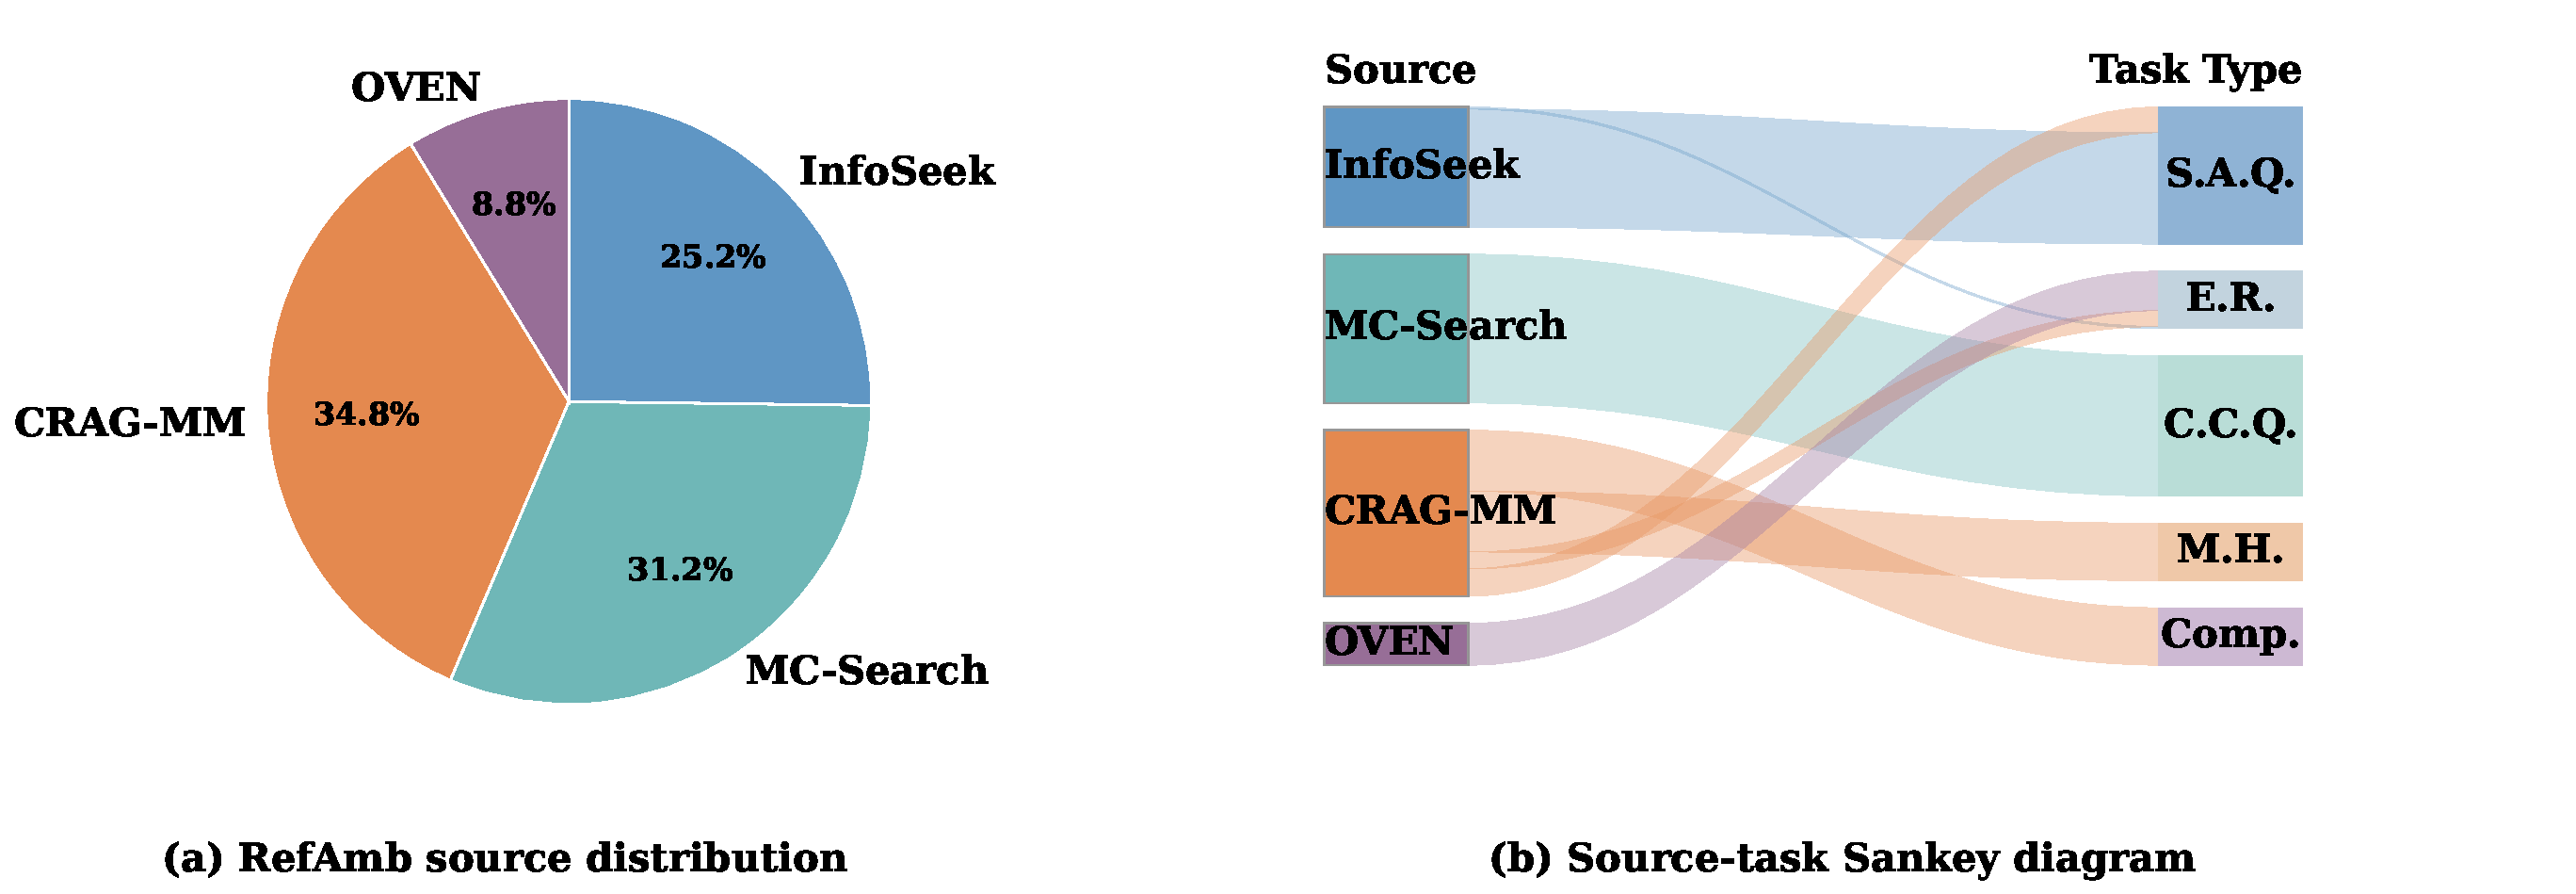
\includegraphics[width=\linewidth]{refamb_original_balanced_source_pie_sankey_combined.pdf}
    \caption{
    Composition of RefAmb.
    (a) shows source composition of the 1,500-sample analysis subset, and the (b) shows task-type composition under our unified diagnostic taxonomy.
    Each task type contains 300 samples for controlled task-balanced analysis.
    }
    \label{fig:dataset-composition}
\end{figure}
As shown in Figure~\ref{fig:dataset-composition}, source composition remains heterogeneous, with CRAG-MM contributing the largest shareIt reflecting that the dataset covers the most comprehensive reasoning forms for question answering.

\subsection{Cross Source Equivalence Test}
To measure the data point equivalence of samples with multiple dataset sources within the same Task Type, we conducted \textbf{TOST} tests on task categories with multi‑source samples, namely Single‑hop Attribute Query and Entity Recognition. As illustrated in Table~\ref{tab:cross_source_consistency_one_table}, within-task cross-source consistency is metric-dependent rather than universal. For Single-hop Attribute Query, question length and external-evidence dependence are equivalent across sources, but answer length, text-alone identifiability, and model-behavior metrics (RTE/LJ) are not. For Entity Recognition, only question length shows robust equivalence, whereas most other properties---especially RTE, LJ, and OK-state ratio---fail equivalence for most source pairs. Therefore, task-type balancing alone does not fully remove source effects; downstream comparisons should still control for source. 

\begin{table}[htbp]
    \centering
    \caption{Cross-source equivalence within task type across practical margins (TOST, $\alpha=0.05$). Each cell reports equivalent source-pairs over all available source-pairs, with the corresponding proportion in parentheses.}
    \begin{tabular}{lccc}
    \toprule
    \textbf{Metric} & \textbf{Margin} & \textbf{S.A.Q.} &\textbf{ E.R.} \\
    \midrule
    $C_1$ Ratio & $\pm0.15$ & 1/1 & 3/3 \\
    $C_2$ Ratio & $\pm0.15$ & 1/1 & 1/3 \\
    \bottomrule
    \end{tabular}
    \label{tab:cross_source_consistency_one_table}
\end{table}

Using multiple sources for the same diagnostic regime increases the diversity of surface forms, visual contexts, answer distributions, and evidence requirements within that regime, thereby reducing the risk that our observations are artifacts of a single dataset construction. However, since different sources may still encode different annotation protocols and difficulty profiles, we interpret task-type differences as source-aware diagnostic patterns rather than source-invariant causal effects.

\section{Experiment Setup Details}\label{app:experiment_setup_details}
We evaluate a ReAct‑style pipeline using Qwen2.5‑VL‑7B‑Instruct as the backbone models for main experiments, and Qwen family models including Qwen3‑VL‑32B‑Instruct and Qwen3.5‑7B for cross‑performance model validation within the same family, as well as InternVL3.5-8B~\citep{wang2025internvl3_5} and BLIP2‑Flan‑T5‑XL~\citep{li2023blip,chung2024scaling} for cross‑family model validation. We reproduce ReAct on FlashRAG~\citep{jin2025flashrag} and reengineered the prior ReAct implementation from ~\citep{li2024benchmarking}. Specially, we restrict the action space to textual and image retrieval while enhancing trajectory robustness by llm output pruning. Each iteration proceeds through: action generation, action parsing, conditional retrieval, evidence injection, and subsequent generation. We set the maximum iteration rounds to 5. The full trajectory—including all triggered actions, inputs/outputs, and overall trajectory states—is meticulously logged to facilitate interventions via static query rewriting and context restoration. Trajectory states are categorized as \textbf{OK}, \textbf{Max-Turn Reached}, or \textbf{Generation Error} induced by context overflow.

\subsection{Trajectory Recording of ReAct Pipeline}
We structured the ReAct reasoning process by requiring the VLM to generate outputs in XML format, mapping each XML tag to a corresponding trajectory node: \texttt{Thought}, \texttt{Sub-question}, \texttt{Search}, and \texttt{Final Answer}, while recording the content associated with each node. Trajectory states were also annotated as follows: \texttt{OK}, indicating successful attainment of the \texttt{Final Answer}; \texttt{Max-Turn reached}, representing trajectories exceeding the maximum number of iterations; and \texttt{GE}, denoting reasoning errors due to context overflow. In the latter two cases, we prompted the LLM to summarize the preceding trajectory and produce the conclusions already discovered as the final answer.
\subsection{LLM Annotation Consistency with Human Annotations}
We report the consistency between the results of LLM‑based annotation for the occurrence of referential ambiguity and human annotations. We also conduct a consistency analysis between the RTE values in our proposed new metric, the Utility judged by the LLM, and human annotations. We employ GPT‑4o for the annotation task, and the consistency analysis results in Table~\ref{tab:human_alignment_rte_refamb} show that annotations by GPT-4o are highly consistent with human annotations.
\begin{table}[htbp]
\centering
\caption{Alignment between human judgments and the proposed RTE. Trajectory-level alignment is measured by rank correlation between human overall labels and RTE. Step-level alignment is measured by binarizing human usefulness labels and model utility scores on all shared annotated steps.}
\label{tab:human_alignment_rte_refamb}
\begin{tabular}{lcc}
\toprule
\textbf{Evaluation Level} & \textbf{Metric} & \textbf{Value} \\
\midrule
Trajectory-level Quality& Spearman's $\rho$ & 0.7061 \\
Trajectory-level Quality& Kendall's $\tau$ & 0.6467 \\
Step-level Utility & Fleiss's $\kappa$ & 0.7198 \\
\midrule
Referential Ambiguity Binary Label & Fleiss's $\kappa$ & 0.8225 \\
% Referential Ambiguity Fined-Grained Label & Fleiss's $\kappa$ & 0.7603 \\
\bottomrule
\end{tabular}
\end{table}
\section{Entity Ambiguity Frequency Across Different VLM Backbones}
% \begin{figure}[htbp]
%     \centering
%     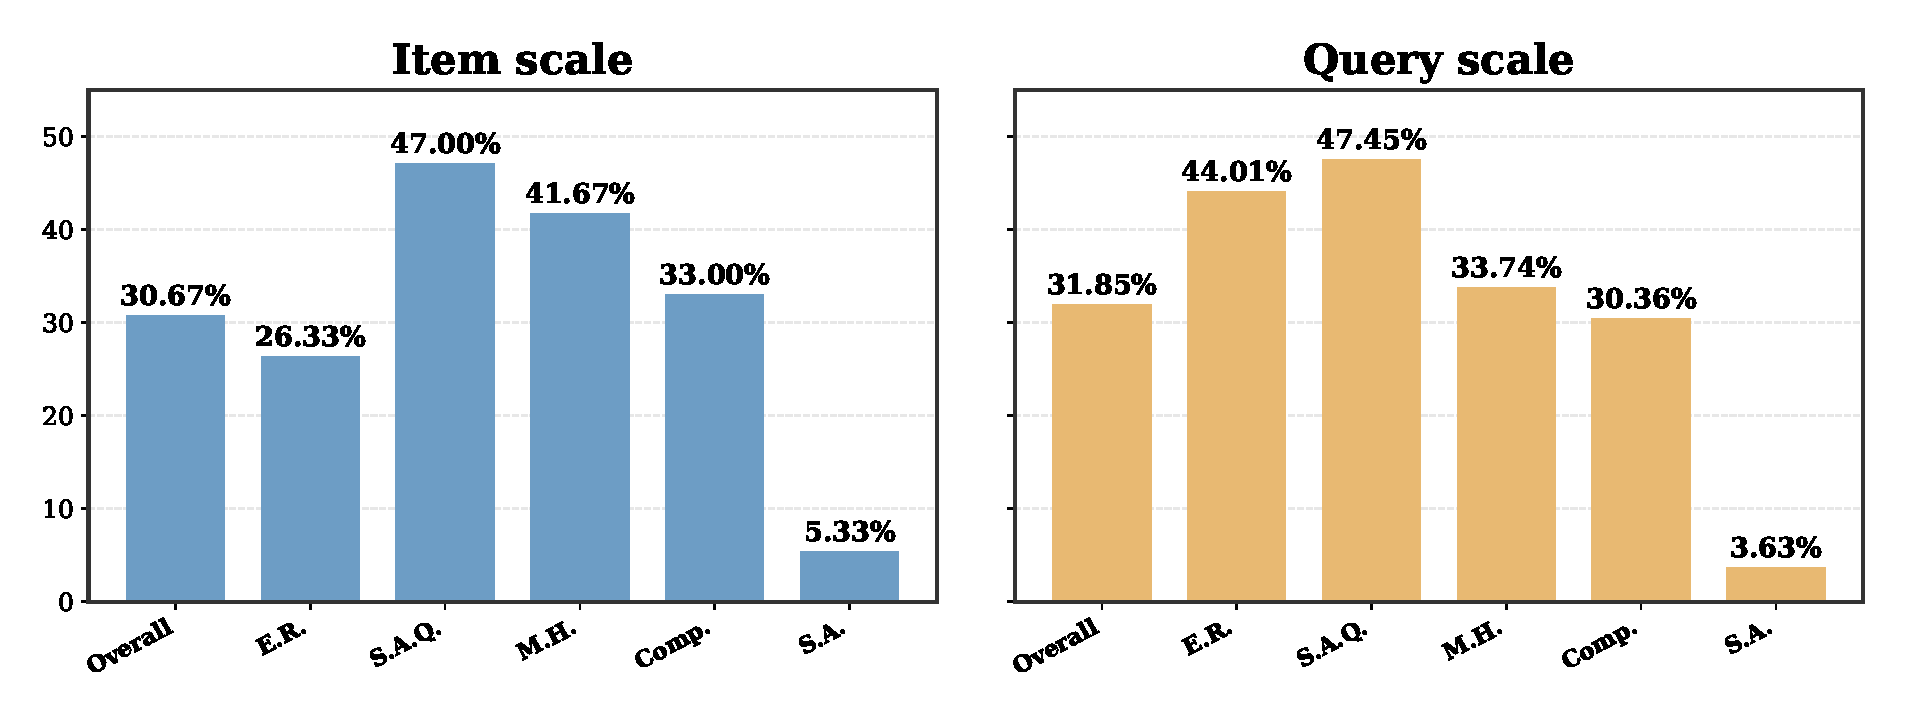
\includegraphics[width=\linewidth]{ambiguity_frequency_by_task_type.pdf}
%     \caption{Referential ambiguity frequency in RefAmb by task type. Ambiguity is frequent overall, but its prevalence varies sharply with task structure and referential dependence.}
%     \label{fig:ambiguity-frequency}
% \end{figure}
Table~\ref{tab:ambiguity_frequency_task_type} reports the frequency of referential ambiguity for additional backbone models, now disaggregated by task type. At the item level, an item is considered ambiguous if at least one labeled retrieval query within its trajectory is entity-ambiguous. At the query level, the frequency is computed as the ratio of entity-ambiguous labeled retrieval queries to the total number of labeled retrieval queries across all items. Referential ambiguity appears consistently across models of different families and scales, as well as across diverse VQA tasks. Some models, such as LLaVA1.5-7B, exhibit very low ambiguity frequency, likely due to their limited ability to interpret and adhere to prompt instructions, often generating text that deviates from the provided cues. InternVL3.5-8B exhibits a high frequency of ambiguous references. This indicates that ambiguous reference is a common issue across models rather than a unique characteristic of a single model. We further validated cross-scale behavior in the Qwen3.5 family: while the 4B and 27B variants display very low probability of entity ambiguity, the 9B variant exhibits substantially higher likelihood.
% \begin{table}[htbp]
% \centering
% \begin{threeparttable}
% \scriptsize
% \setlength{\tabcolsep}{3pt}
% \caption{Entity ambiguity frequency across backbone models and task types. Each model is evaluated on RefAmb subset, and the same task-type decomposition is applied across backbones.}
% \begin{tabular}{llrrrrrr}
% \toprule
% \textbf{Model} & \textbf{Task Type} & \textbf{Items} & \textbf{Amb. Items} & \textbf{Item \%} & \textbf{Queries} & \textbf{Amb. Queries} & \textbf{Query \%} \\
% \midrule
% Qwen2.5-VL-7B & Overall & 1500 & 460 & 30.67\% & 4433 & 1412 & 31.85\% \\
% Qwen2.5-VL-7B & Entity Recognition & 300 & 79 & 26.33\% & 534 & 235 & 44.01\% \\
% Qwen2.5-VL-7B & Single-hop Attribute Query & 300 & 141 & 47.00\% & 999 & 474 & 47.45\% \\
% Qwen2.5-VL-7B & Multi-hop & 300 & 125 & 41.67\% & 1070 & 361 & 33.74\% \\
% Qwen2.5-VL-7B & Comparison & 300 & 99 & 33.00\% & 1031 & 313 & 30.36\% \\
% Qwen2.5-VL-7B & Subproblem Aggregation & 300 & 16 & 5.33\% & 799 & 29 & 3.63\% \\
% \midrule
% LLaVA1.5-7B & Overall & 1500 & 8 & 0.53\% & 1172 & 8 & 0.68\% \\
% LLaVA1.5-7B & Entity Recognition & 300 & 0 & 0.00\% & 160 & 0 & 0.00\% \\
% LLaVA1.5-7B & Single-hop Attribute Query & 300 & 3 & 1.00\% & 205 & 3 & 1.46\% \\
% LLaVA1.5-7B & Multi-hop & 300 & 1 & 0.33\% & 238 & 1 & 0.42\% \\
% LLaVA1.5-7B & Comparison & 300 & 2 & 0.67\% & 185 & 2 & 1.08\% \\
% LLaVA1.5-7B & Subproblem Aggregation & 300 & 2 & 0.67\% & 384 & 2 & 0.52\% \\
% \midrule
% InternVL3.5-8B & Overall & 1500 & 694 & 46.27\% & 2604 & 1062 & 40.78\% \\
% InternVL3.5-8B & Entity Recognition & 300 & 148 & 49.33\% & 425 & 224 & 52.71\% \\
% InternVL3.5-8B & Single-hop Attribute Query & 300 & 217 & 72.33\% & 741 & 473 & 63.83\% \\
% InternVL3.5-8B & Multi-hop & 300 & 158 & 52.67\% & 357 & 176 & 49.30\% \\
% InternVL3.5-8B & Comparison & 300 & 143 & 47.67\% & 351 & 155 & 44.16\% \\
% InternVL3.5-8B & Subproblem Aggregation & 300 & 28 & 9.33\% & 730 & 34 & 4.66\% \\
% \midrule
% Qwen3.5-4B & Overall & 500 & 37 & 7.40\% & 993 & 47 & 4.73\% \\
% Qwen3.5-4B & Entity Recognition & 100 & 16 & 16.00\% & 138 & 23 & 16.67\% \\
% Qwen3.5-4B & Single-hop Attribute Query & 100 & 5 & 5.00\% & 211 & 8 & 3.79\% \\
% Qwen3.5-4B & Multi-hop & 100 & 7 & 7.00\% & 185 & 7 & 3.78\% \\
% Qwen3.5-4B & Comparison & 100 & 6 & 6.00\% & 241 & 6 & 2.49\% \\
% Qwen3.5-4B & Subproblem Aggregation & 100 & 3 & 3.00\% & 218 & 3 & 1.38\% \\
% \midrule
% Qwen3.5-9B & Overall & 500 & 110 & 22.00\% & 1040 & 151 & 14.52\% \\
% Qwen3.5-9B & Entity Recognition & 100 & 31 & 31.00\% & 144 & 41 & 28.47\% \\
% Qwen3.5-9B & Single-hop Attribute Query & 100 & 30 & 30.00\% & 193 & 45 & 23.32\% \\
% Qwen3.5-9B & Multi-hop & 100 & 25 & 25.00\% & 263 & 34 & 12.93\% \\
% Qwen3.5-9B & Comparison & 100 & 23 & 23.00\% & 236 & 30 & 12.71\% \\
% Qwen3.5-9B & Subproblem Aggregation & 100 & 1 & 1.00\% & 204 & 1 & 0.49\% \\
% \midrule
% Qwen3.5-27B & Overall & 500 & 21 & 4.20\% & 1264 & 27 & 2.14\% \\
% Qwen3.5-27B & Entity Recognition & 100 & 7 & 7.00\% & 165 & 8 & 4.85\% \\
% Qwen3.5-27B & Single-hop Attribute Query & 100 & 7 & 7.00\% & 240 & 9 & 3.75\% \\
% Qwen3.5-27B & Multi-hop & 100 & 3 & 3.00\% & 301 & 6 & 1.99\% \\
% Qwen3.5-27B & Comparison & 100 & 1 & 1.00\% & 277 & 1 & 0.36\% \\
% Qwen3.5-27B & Subproblem Aggregation & 100 & 3 & 3.00\% & 281 & 3 & 1.07\% \\
% \bottomrule
% \end{tabular}
% \label{tab:appendix-ambiguity-frequency-by-model-and-task-type}
% \end{threeparttable}
% \end{table}
\begin{table}[htbp]
    \centering
    \setlength{\tabcolsep}{3pt}
    \caption{Entity ambiguity frequency across backbone models and natural dataset distrubutions.}
    \begin{tabular}{l c c c c c c c c}
    \hline
    \textbf{Model} & \multicolumn{2}{c}{\textbf{CRAG-MM}} & \multicolumn{2}{c}{\textbf{InfoSeek}} & \multicolumn{2}{c}{\textbf{MCSearch}} & \multicolumn{2}{c}{\textbf{OVEN}} \\
    \cline{2-3} \cline{4-5} \cline{6-7} \cline{8-9}
    & Item & Query & Item & Query & Item & Query & Item & Query \\
    \midrule
    InternVL3.5-8B & 48.90 & 46.05 & 90.91 & 70.07 & 9.67 & 4.66 & 52.43 & 52.30 \\
    LLaVA1.5-7B & 1.22 & 0.71 & 1.14 & 1.61 & 0.67 & 0.52 & 0.00 & 0.00 \\
    Qwen2.5-VL-7B & 36.92 & 33.24 & 56.82 & 56.89 & 5.33 & 3.63 & 22.33 & 42.90 \\
    Qwen3-VL-32B & 7.70 & 3.90 & 12.50 & 11.64 & 1.33 & 0.74 & 6.80 & 7.34 \\
    Qwen3-VL-4B & 21.52 & 16.72 & 69.32 & 47.12 & 4.67 & 1.76 & 35.92 & 35.14 \\
    Qwen3-VL-8B & 23.84 & 15.94 & 60.80 & 44.02 & 4.33 & 1.74 & 31.07 & 33.67 \\
    Qwen3.5-4B  & 6.25 & 3.60 & 9.26 & 4.46 & 3.00 & 1.38 & 14.19 & 15.79 \\
    Qwen3.5-9B  & 23.90 & 14.98 & 33.33 & 22.05 & 1.00 & 0.49 & 35.14 & 28.70 \\
    Qwen3.5-27B  & 2.94 & 1.66 & 9.26 & 4.67 & 3.00 & 1.07 & 6.76 & 4.50 \\
    \midrule
    \end{tabular}
    \label{tab:ambiguity_frequency_source}
\end{table}

\begin{table}[htbp]
\centering
% \scriptsize
\setlength{\tabcolsep}{3pt}
\caption{Entity ambiguity frequency across backbone models and task types.}
\begin{tabular}{l c c c c c c c c c c c c}
\toprule
\multirow{2}{*}{\textbf{Model}} & 
\multicolumn{2}{c}{\textbf{Overall}} &
\multicolumn{2}{c}{\textbf{E.R.}} &
\multicolumn{2}{c}{\textbf{S.A.Q.}} &
\multicolumn{2}{c}{\textbf{M.H.}} &
\multicolumn{2}{c}{\textbf{Comp.}} &
\multicolumn{2}{c}{\textbf{S.A.}} \\
\cmidrule(lr){2-3} \cmidrule(lr){4-5} \cmidrule(lr){6-7} \cmidrule(lr){8-9} \cmidrule(lr){10-11} \cmidrule(lr){12-13}
 & Item  & Query  & Item  & Query  & Item  & Query  & Item  & Query  & Item  & Query  & Item  & Query  \\
\midrule
Qwen2.5-VL-7B & 30.67 & 31.85 & 26.33 & 44.01 & 47.00 & 47.45 & 41.67 & 33.74 & 33.00 & 30.36 & 5.33 & 3.63 \\
Qwen3-VL-2B & 0.00 & 0.00 & 0.00 & 0.00 & 0.00 & 0.00 & 0.00 & 0.00 & 0.00 & 0.00 & 0.00 & 0.00 \\
Qwen3-VL-4B & 25.73 & 19.84 & 35.67 & 34.24 & 44.67 & 37.36 & 21.67 & 16.93 & 22.00 & 15.13 & 4.67 & 1.80 \\
Qwen3-VL-8B & 25.27 & 18.81 & 31.33 & 32.57 & 47.33 & 38.65 & 22.33 & 13.02 & 21.00 & 12.88 & 4.33 & 1.72 \\
Qwen3-VL-32B & 6.87 & 4.24 & 10.33 & 11.62 & 9.33 & 8.98 & 9.00 & 3.36 & 4.33 & 2.65 & 1.33 & 0.75 \\
Qwen3.5-4B & 7.40 & 4.73 & 16.00 & 16.67 & 5.00 & 3.79 & 7.00 & 3.78 & 6.00 & 2.49 & 3.00 & 1.38 \\
Qwen3.5-9B & 22.00 & 14.52 & 31.00 & 28.47 & 30.00 & 23.32 & 25.00 & 12.93 & 23.00 & 12.71 & 1.00 & 0.49 \\
Qwen3.5-27B & 4.20 & 2.14 & 7.00 & 4.85 & 7.00 & 3.75 & 3.00 & 1.99 & 1.00 & 0.36 & 3.00 & 1.07 \\
LLaVA1.5-7B & 0.53 & 0.68 & 0.00 & 0.00 & 1.00 & 1.46 & 0.33 & 0.42 & 0.67 & 1.08 & 0.67 & 0.52 \\
InternVL3.5-8B & 46.27 & 40.78 & 49.33 & 52.71 & 72.33 & 63.83 & 52.67 & 49.30 & 47.67 & 44.16 & 9.33 & 4.66 \\
\bottomrule
\end{tabular}
\label{tab:ambiguity_frequency_task_type}
\end{table}

\section{Details on RTE}
\subsection{Partial Contrubution Label Value Sensitivity}
We also conduct hyper‑parameter sensitivity analysis for partial contribution label values in the calculation of $U_t$ within the RTE system, with values ranging from 0.1 to 0.9. Subsequently, we estimate the consistency between the RTE values obtained from different partial values and human evaluations of trajectory quality, using Spearman and Kendall correlation coefficients to quantify the degree of consistency. The results are shown in Figure~\ref{fig:human_alignment_partial_contribution_sensitivity.pdf}.

\begin{figure}[htbp]
    \centering
    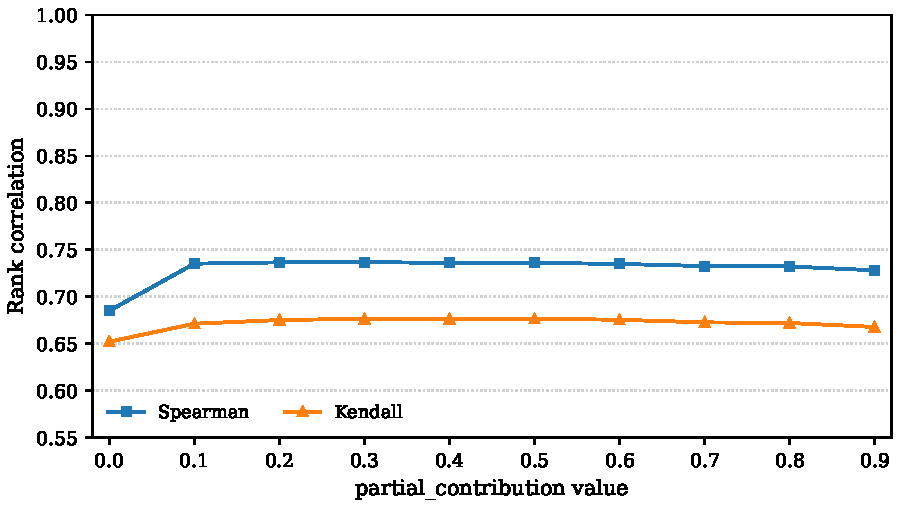
\includegraphics[width=0.8\linewidth]{human_alignment_partial_contribution_sensitivity.pdf}
    \caption{Hyper-parameters sensitive analysis for partial contrubution label value.}
    \label{fig:human_alignment_partial_contribution_sensitivity.pdf}
\end{figure}

It can be seen from the figure that the value of partial value has a weak impact on the final consistency, with a flat curve. Consistency only decreases when partial value is 0, the same as no contribution, and there is a slight decrease when the value approaches 1 of full contribution. This reflects the importance of the level of partial contribution.
\subsection{Correlation between RTE and Generation Quality}
As shown in Table~\ref{tab:rte-gptacc-corr-auc}, both Pearson and Spearman correlation coefficients indicate that higher RTE values are generally associated with a greater probability of correct responses. While the relationship is neither strictly linear nor determinative, a monotonic trend is evident across the dataset. The AUROC further in Table~\ref{tab:rte-gptacc-corr-auc} and Figure~\ref{fig:rte_lj_auroc_curve} confirms that RTE provides a moderate discriminative signal for distinguishing correct from incorrect answers. 
\begin{table}[htbp]
\centering
\begin{minipage}[c]{0.48\textwidth}
  \centering
  \captionof{table}{Correlation and discriminative statistics between RTE and final correctness (GPT-Acc) on the four Original RefAmb sources.}
    \begin{tabular}{lcccc}
    \toprule
     & Pearson $r$ & Spearman $\rho$ & AUROC \\
    \midrule
    Value & 0.3752 & 0.3287 & 0.7054\\
    \bottomrule
    \end{tabular}
    \label{tab:rte-gptacc-corr-auc}
\end{minipage}
\hfill
\begin{minipage}[c]{0.48\textwidth}
  \centering
  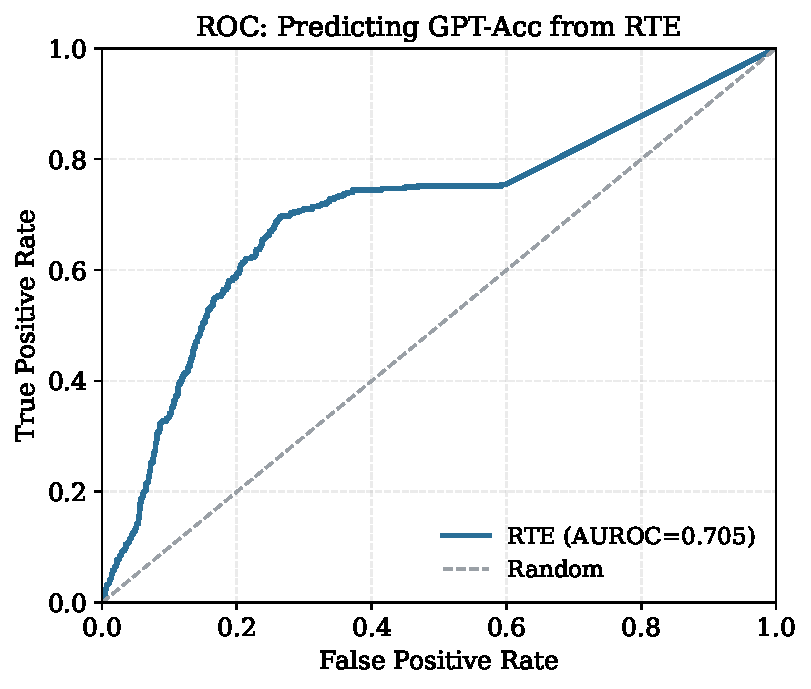
\includegraphics[width=\linewidth]{rte_lj_auroc_curve.pdf}
  \captionof{figure}{The discriminative capability of the trajectory-level RTE metric in predicting final answer correctness.}
  \label{fig:rte_lj_auroc_curve}
\end{minipage}
\end{table}
Overall, these results suggest that RTE can moderately reflect answer correctness, though it is not strongly predictive. This limitation arises from the inherent complexity of real-world questions and the influence of hallucinated knowledge, which can lead to highly active pipeline trajectories that nevertheless produce incorrect outputs.
\section{Intervention Experiments Details}
\begin{figure}[htbp]
    \centering
    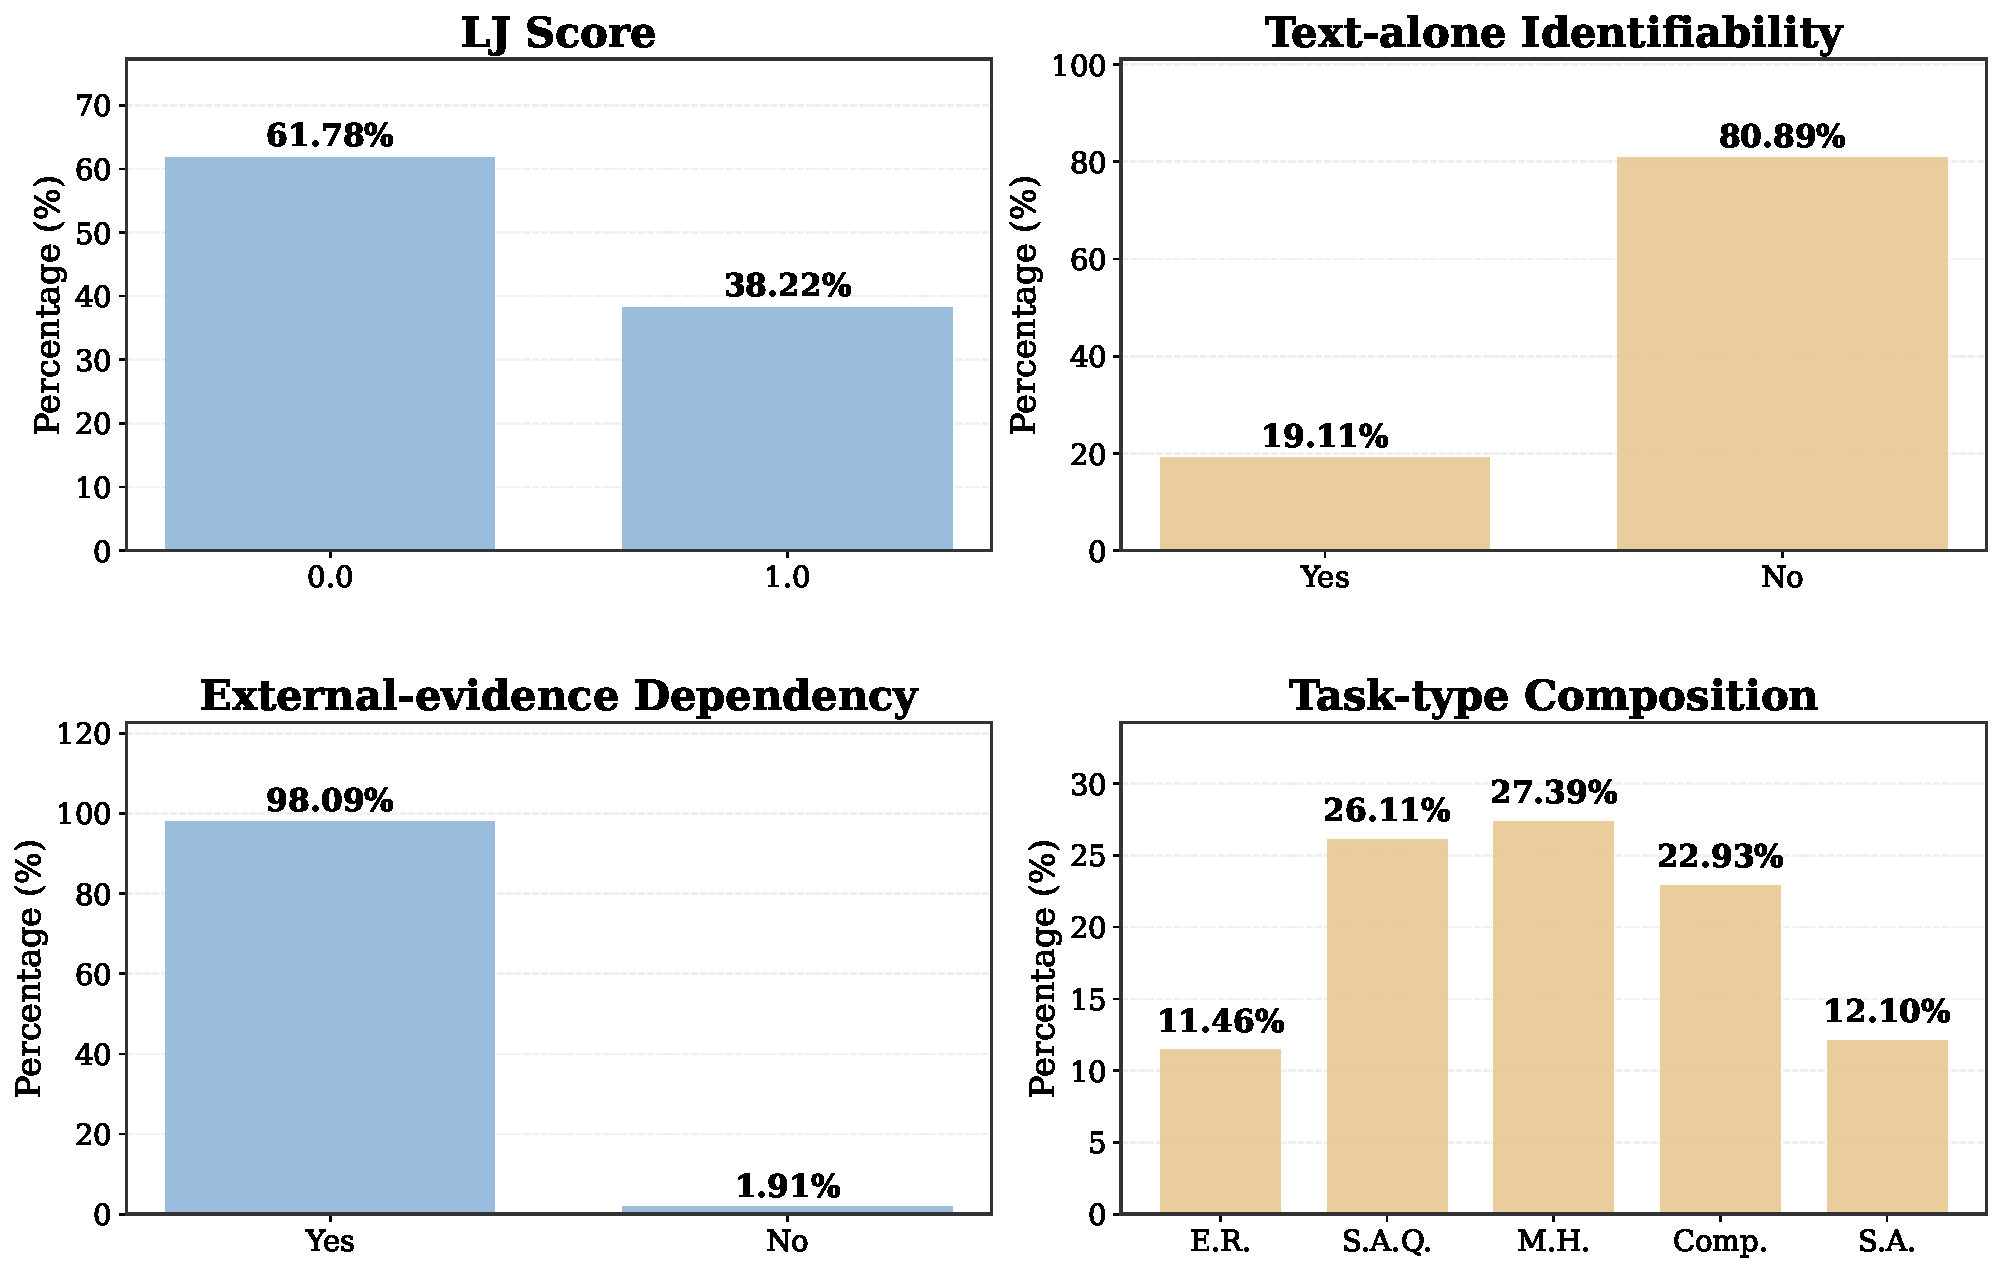
\includegraphics[width=0.9\linewidth]{disturb_failure_to_ok_composition.pdf}
    \caption{Distribution of Disturb-recovered items (157 in total), including answer correctness, text-only identifiability, external-evidence dependence, and task-type composition.}
    \label{fig:disturb_failure_to_ok_composition}
\end{figure}
\subsection{Properties of Disturb-Recovered Items}
We extracted whole items (157) from the Disturb Intervention in which the trajectory state transitioned from \texttt{generation error} or \texttt{max turn reached} to \texttt{OK}, and analyzed these items with respect to task type, final answer correctness, modality coupling of the questions $C_1$, and dependence on external knowledge $C_2$. Figure~\ref{fig:disturb_failure_to_ok_composition} summarizes the composition of the recovered items. The analysis reveals that, despite the trajectory status being restored to \texttt{OK}, the generated answers remain largely erroneous. Furthermore, items whose state could be recovered predominantly exhibit strong modality coupling and high reliance on external knowledge. This observation corroborates that the Disturb intervention enhances trajectory activity under conditions requiring real-world knowledge retrieval, yet does not effectively translate into commensurate gains in final generation quality. Among the recovered items, multi-hop tasks, comparison tasks, and entity attribute queries are most prevalent, corresponding to the categories with the strongest modality coupling and external knowledge dependency, as illustrated in Figure~\ref{fig:stage1-label-2d-by-task-type}.
\subsection{Oracle Intervention Details}
Figure~\ref{fig:oracle-transition} summarizes the dynamic effects of Oracle intervention on trajectory states. 
\begin{wrapfigure}{r}{0.5\textwidth}
    \centering
    
\includegraphics[width=0.5\textwidth]{first_round_oracle_rewrite_transition_focus.pdf}
    \caption{First-round Oracle rewrite state transitions.}
    \label{fig:oracle-transition}
\end{wrapfigure}
Most failed trajectories are recovered to the OK state, indicating that Oracle can redirect failing reasoning chains by supplying precise entity grounding. Trajectories that were originally OK largely persist, although a smaller subset regresses. The stacked bar chart quantifies these transitions and shows that Oracle can both repair failures and perturb some already stable paths.
\subsection{Analysis of More Indicator Results Under Two Intervention Settings}
\begin{figure}[htbp]
    \centering
    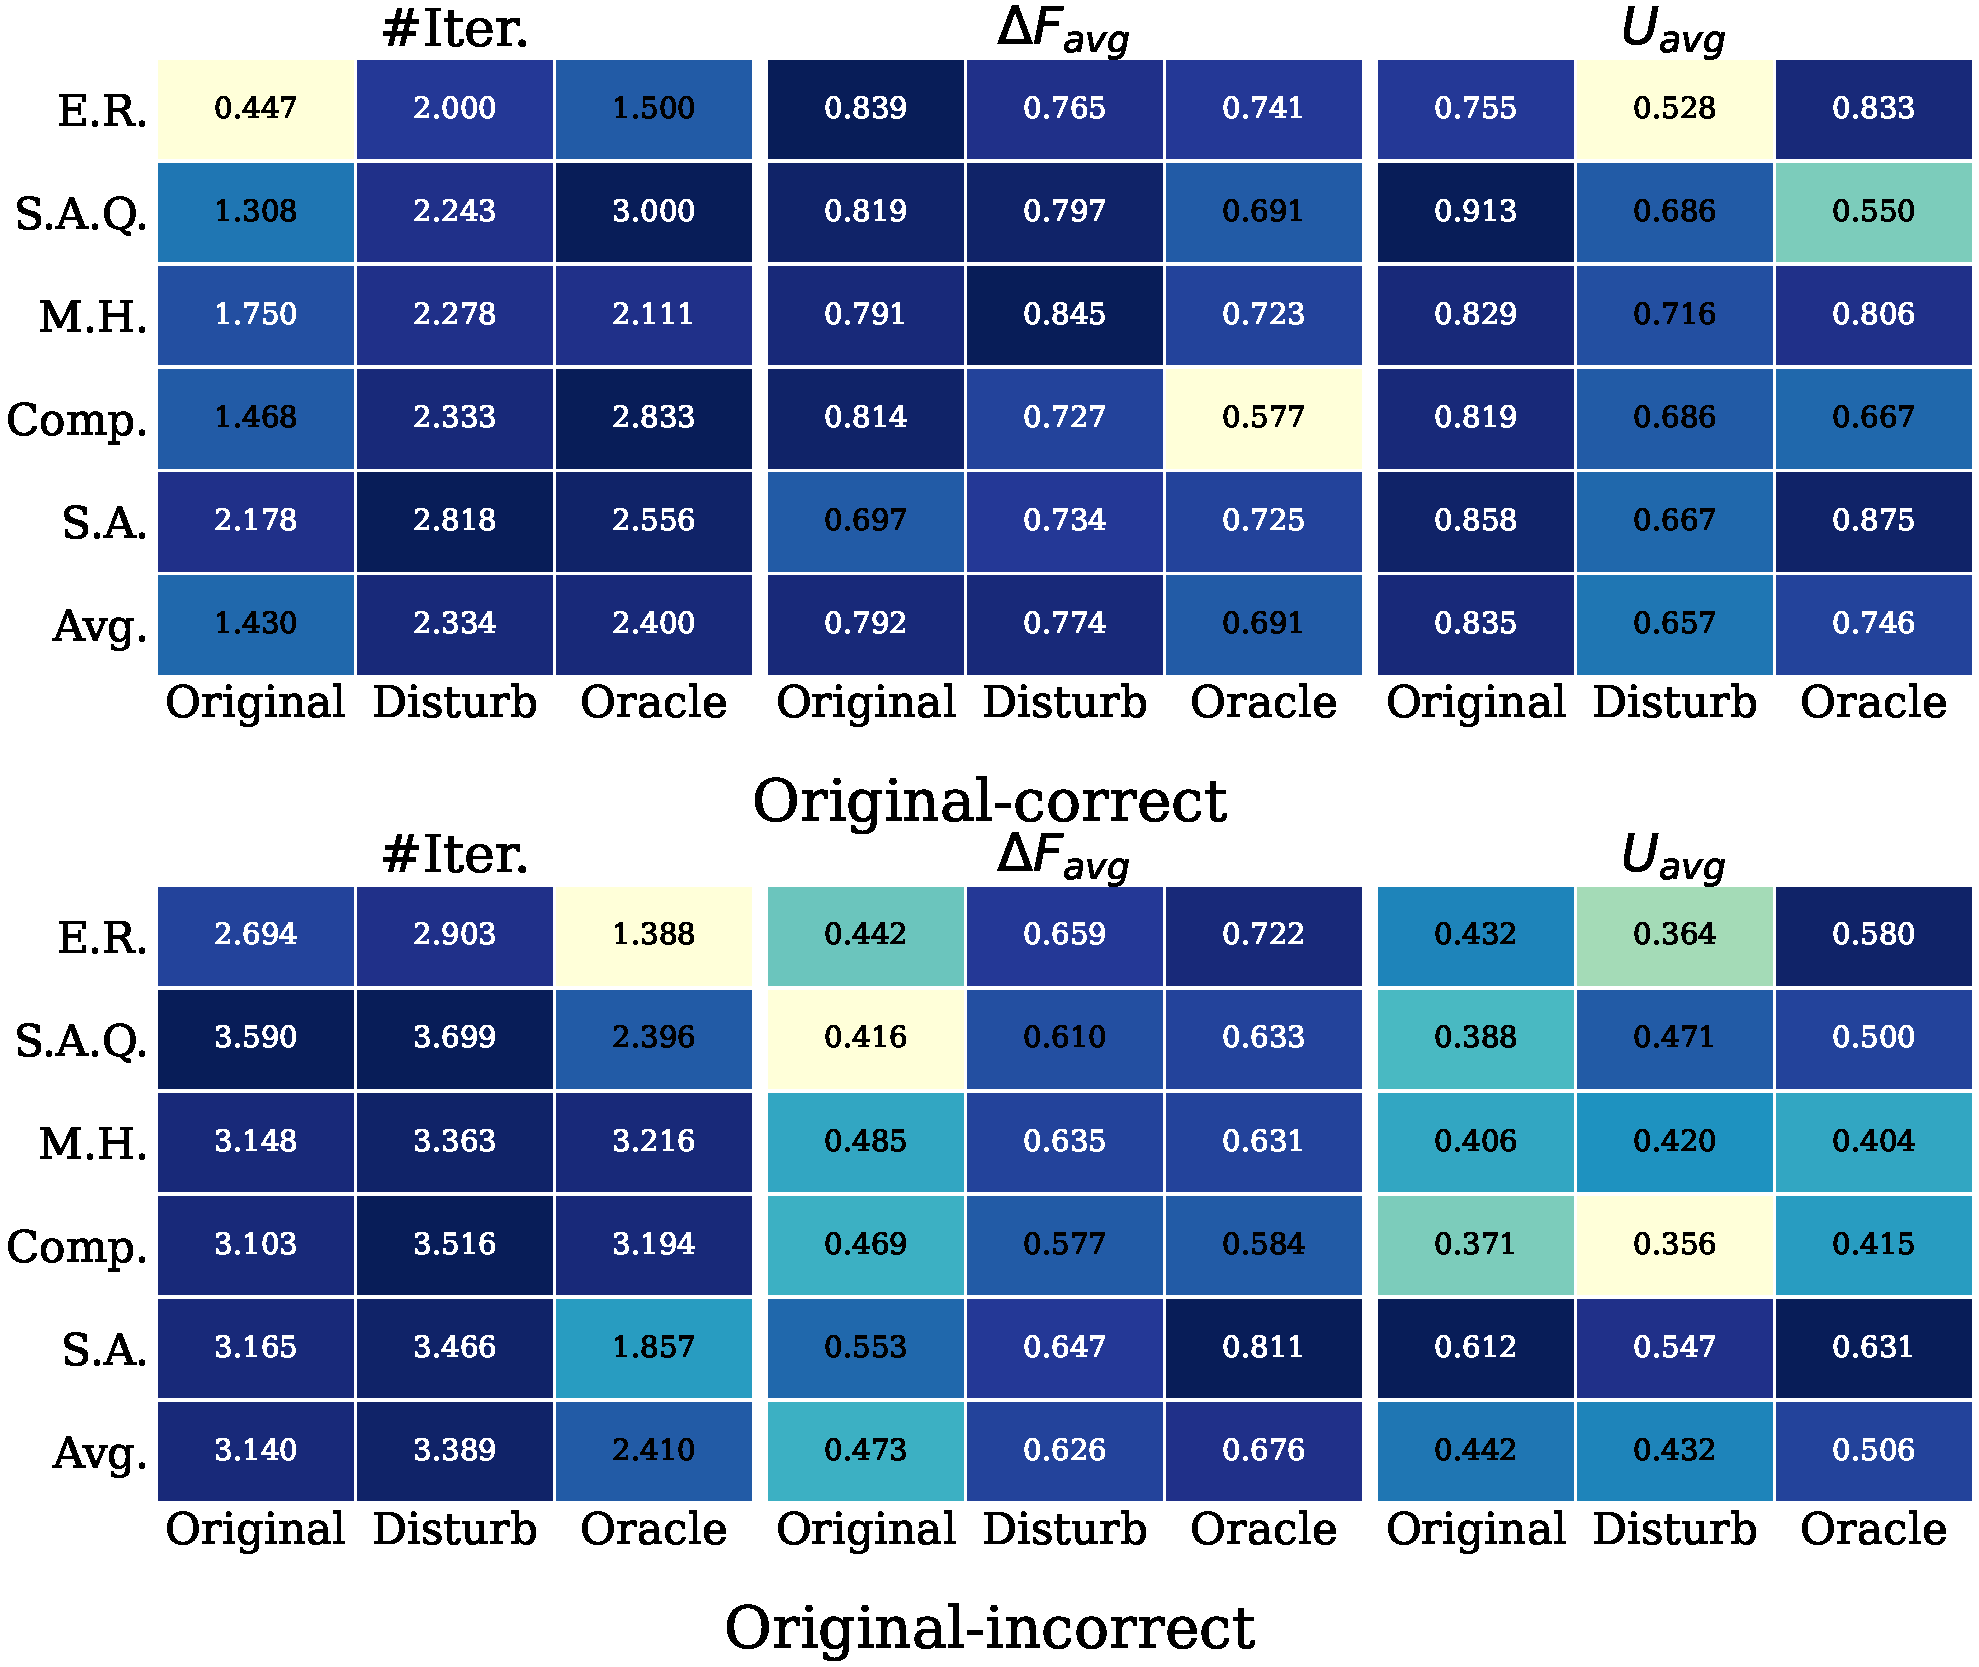
\includegraphics[width=0.7\linewidth]{trajectory_quality_appendix_heatmap.pdf}
    \caption{Average step-level iterations (\#Iter.), information increment ($\Delta F_\text{avg}$), and utility ($U_\text{avg}$) for Original, Disturb, and Oracle across task types.}
    \label{fig:trajectory_quality_appendix_heatmap}
\end{figure}
In addition to reporting the RTE metric, we also recorded the step-level information increment $\Delta F$ and utility $U$ to enable a more fine-grained analysis of trajectory activity, as illustrated in Figure~\ref{fig:trajectory_quality_appendix_heatmap}. For samples that were already correctly answered by the original pipeline, neither intervention produced substantial changes in $\Delta F$ or $U$ across iterations; however, both interventions yielded slightly lower $\Delta F$ and utility values compared to the original trajectory. For originally incorrect samples, both Disturb and Oracle increased the information richness of retrieved evidence, with Oracle generally showing the larger improvement in aggregate.
\subsection{Source-Level Intervention Effects}
Due to the construction characteristics of RefAmb, populating different task types from multiple datasets ensures the diversity of samples within each task category but inevitably introduces dataset-distribution bias.
Therefore, analyzing the two intervention methods from the perspective of task types will unavoidably bring in additional source-related factors.
Nevertheless, the source-level view is still informative because it reveals the same broad pattern seen in the cross-model validation: the interventions are not uniformly beneficial.
As illustrated in Figure~\ref{fig:trajectory_quality_by_source}, both Oracle and Disturb can improve trajectory activity on some sources, but Disturb does not consistently translate into better generation quality.
The source breakdown also shows that MCSearch is especially sensitive to query reformulation, whereas OVEN can remain relatively stable even when Oracle changes the initial query.
These differences reinforce the interpretation that query specificity is a controllable signal, but only within a limited operating region defined by the source and the backbone.
\begin{figure}
    \centering
    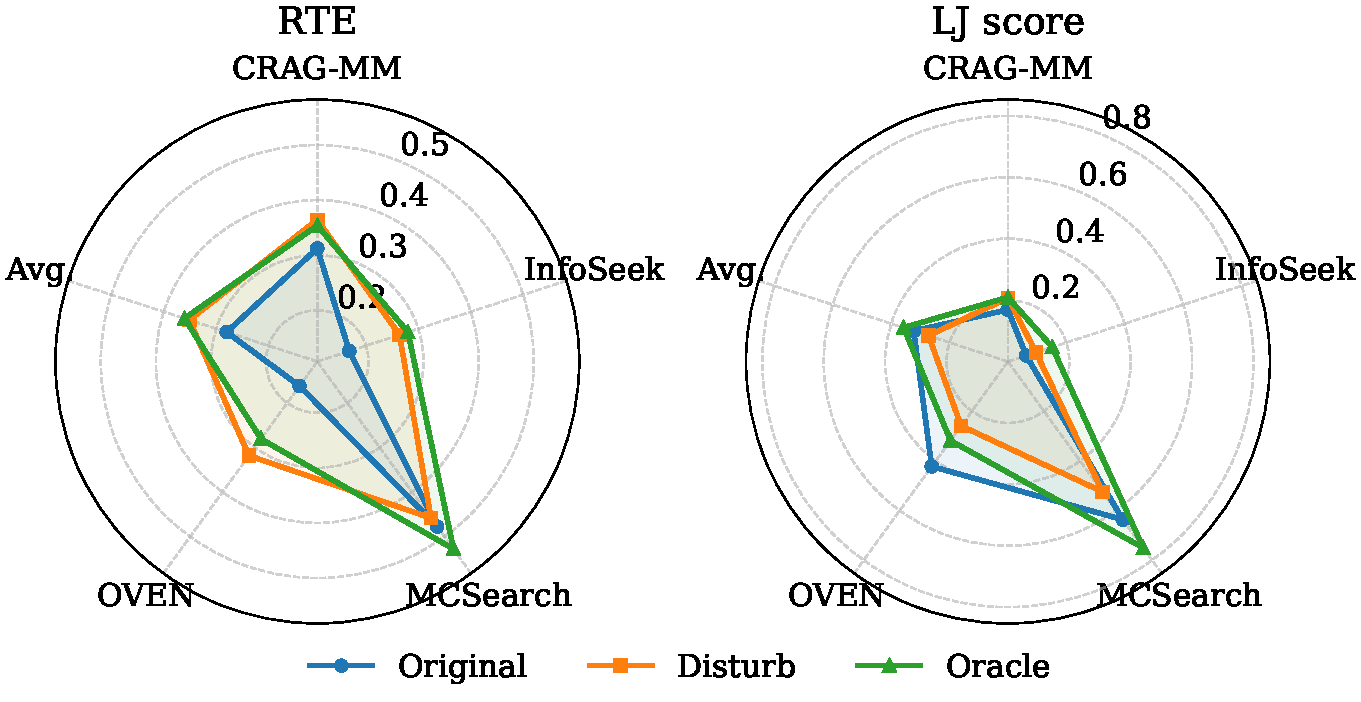
\includegraphics[width=0.9\linewidth]{trajectory_quality_by_source.pdf}
    \caption{Trajectory dynamics and generation quality under the two interventions from a source-aware perspective.}
    \label{fig:trajectory_quality_by_source}
\end{figure}
\subsection{Statistical Robustness and Boundary Checks}
Because a full specificity sweep would require additional API calls over the entire 1,500-item benchmark, we validate the main claim with three low-cost checks on the existing outputs: paired bootstrap estimates, natural ambiguity bins, and cross-backbone transfer.
At the answer level, the bootstrap confidence intervals confirm that Oracle is consistently positive while Disturb is near-neutral or negative depending on the backbone.
For example, the paired delta in accuracy is $+0.052$ \,[0.028, 0.076] for Qwen2.5-VL-7B under Oracle, $+0.102$ \,[0.078, 0.127] for InternVL3.5-8B, $+0.081$ \,[0.050, 0.112] for Qwen3-VL-4B, $+0.063$ \,[0.032, 0.095] for Qwen3-VL-8B, and $+0.087$ \,[0.029, 0.155] for Qwen3-VL-32B.
By contrast, Disturb is approximately neutral on Qwen2.5-VL-7B ($+0.001$ \,[$-0.005$, 0.007]) and InternVL3.5-8B ($+0.002$ \,[$-0.007$, 0.012]), but slightly negative on the Qwen3 family (around $-0.003$ to $-0.005$).
The paired transition rates tell the same story: Oracle consistently raises the failure-to-OK repair rate and keeps the regression rate lower than the repair rate, while Disturb only produces a modest repair gain on Qwen2.5 and becomes mostly regression-prone on Qwen3.
At the trajectory level, the natural ambiguity bins provide a proxy sweep: in the macro-average split, ambiguous queries have lower RTE than non-ambiguous queries in both the correct subset ($0.515$ vs.\ $0.676$) and the incorrect subset ($0.186$ vs.\ $0.302$), while also requiring more iterations.
This means that reducing ambiguity is not automatically equivalent to improving trajectory quality, but it does shift the trajectory into a different operating region.
\subsection{Residual Ambiguity After Oracle Rewrite}
Table~\ref{tab:oracle-rewrite-entity-ambiguity} shows that residual ambiguity remains after Oracle rewrite. Across paired cohorts of original and Oracle-intervened trajectories, items containing at least one entity-ambiguous retrieval step decrease from 100\% to 59.35\%, and ambiguous retrieval steps drop from 77.89\% to 37.00\%. 
The persistence of residual ambiguity indicates that first-round Oracle intervention does not merely rectify a one-off input defect. 
Extended trajectories increase the likelihood of hitting the maximum iteration limit (leading to Max Turn Reached state) or exceeding the model’s context window (leading to Generation Error state), thereby impeding convergence to a final answer. This pattern suggests a mismatch between the VLM and the retriever: the VLM does not fully account for the retriever's interface, preferences, and feedback when generating queries.
\begin{table}[htbp]
\centering
\small
\setlength{\tabcolsep}{6pt}
\caption{Entity ambiguity before and after Oracle rewrite.}
\begin{tabular}{lrrr}
\hline
\textbf{Metric} & \textbf{Before Oracle Rewrite} & \textbf{After Oracle Rewrite} & \textbf{Reduction} \\
\hline
Item Scale & 100.00\% & 59.35\% & 40.65 pct \\
Step Scale & 77.89\% & 37.00\% & 40.90 pct \\
\hline
\end{tabular}
\label{tab:oracle-rewrite-entity-ambiguity}
\end{table}

\section{IIGCR Procedure}\label{app:algorithm}
Algorithm~\ref{alg:eao} formalizes the auxiliary IIGCR loop, which monitors each text-retrieval step and applies two gating mechanisms to detect potential trajectory stagnation: query-similarity stagnation, triggered when consecutive queries exhibit high semantic overlap, and low information-gain stagnation, triggered when step-level information increments fall below a predefined threshold.
\begin{algorithm}[htbp]
\small
\KwIn{Messages $\mathcal{M}$, image $I$, current text query $q_t$, previous accepted text query $q_{t-1}^{\mathrm{ret}}$, history units $\mathcal{H}$}
\KwOut{Updated messages $\mathcal{M}$}
\textbf{Initialize:} $r\leftarrow 0$, $s_{\mathrm{sim}}\leftarrow 0$, $s_{\mathrm{gain}}\leftarrow 0$;

\tcp{Gate A: query-similarity stagnation}
\If{$q_{t-1}^{\mathrm{ret}}\neq\varnothing$ \textbf{and} $\mathrm{sim}(q_t,q_{t-1}^{\mathrm{ret}})>\tau_s$}{
    $s_{\mathrm{sim}}\leftarrow s_{\mathrm{sim}}+1$\;
    \uIf{$s_{\mathrm{sim}}\ge 2$}{
        $\mathcal{M}\leftarrow \operatorname{RebuildMessages}(\mathcal{M},\texttt{reflection})$\;
        $\mathcal{M}\leftarrow \operatorname{PruneTrajectoryStates}(\mathcal{M})$\;
        \Return{$\mathcal{M}$}\;
    }
    \uElse{
        $\mathcal{M}\leftarrow \operatorname{RebuildMessages}(\mathcal{M},\texttt{missing\_info})$\;
        \Return{$\mathcal{M}$}\;
    }
}
\Else{
    $s_{\mathrm{sim}}\leftarrow 0$\;
}

\tcp{Execute text retrieval and estimate information gain}
$q_t^{\mathrm{ret}}\leftarrow q_t$\;
$R_t\leftarrow \operatorname{TextRetrieval}(q_t^{\mathrm{ret}})$\;
$\Delta F_t,\,NF\leftarrow \operatorname{NewFactsRatio}(q_t^{\mathrm{ret}},q_{t-1}^{\mathrm{ret}},R_t,\mathcal{H})$\;

\tcp{Gate B: low information-gain stagnation}
\If{$\Delta F_t<\tau_f$}{
    $s_{\mathrm{gain}}\leftarrow s_{\mathrm{gain}}+1$\;
    \uIf{$s_{\mathrm{gain}}\ge 2$}{
        $\mathcal{M}\leftarrow \operatorname{RebuildMessages}(\mathcal{M},\texttt{reflection})$\;
        $\mathcal{M}\leftarrow \operatorname{PruneTrajectoryStates}(\mathcal{M})$\;
        \Return{$\mathcal{M}$}\;
    }
    \uElse{
        $\mathcal{M}\leftarrow \operatorname{RebuildMessages}(\mathcal{M},\texttt{missing\_info})$\;
        \Return{$\mathcal{M}$}\;
    }
}
\Else{
    $s_{\mathrm{gain}}\leftarrow 0$\;
}

\tcp{Accept retrieval and continue}
$q_{t-1}^{\mathrm{ret}}\leftarrow q_t^{\mathrm{ret}}$\;
$\mathcal{H}\leftarrow \mathcal{H}\oplus NF$\;
$r\leftarrow 0,\; s_{\mathrm{sim}}\leftarrow 0$\;
$\mathcal{M}\leftarrow \operatorname{UpdateMessages}(\mathcal{M},R_t)$\;
\Return{$\mathcal{M}$}\;
\caption{ATL-CI Recovery Logic in \texttt{atl\_ci\_ablation.py} (current implementation)}
\label{alg:eao}
\end{algorithm}

\begin{algorithm}[htbp]
\small
\KwIn{Messages $\mathcal{M}$, mode $m\in\{\texttt{missing\_info},\texttt{reflection}\}$, reference query $q$, feedback $f$}
\KwOut{Rebuilt messages $\mathcal{M}'$, rebuilt response $a$}
\uIf{$m=\texttt{missing\_info}$}{
    $a_{raw}\leftarrow \operatorname{BuildMissingInfoRewrite}(q,f)$\;
    $(d,a)\leftarrow \operatorname{InferRebuildDiagnosis}(q,a_{raw},f)$\;
    \tcp*[l]{replace the latest assistant \texttt{<Search>} state in-place}
    \If{latest assistant search node exists in $\mathcal{M}$}{
        replace that node with $a$\;
    }
    \Else{
        append assistant node with $a$\;
    }
    $\mathcal{M}'\leftarrow \mathcal{M}$\;
    \Return{$\mathcal{M}',a$}\;
}
\Else{\tcp*[f]{\texttt{reflection}}
    $(\tilde{\mathcal{M}},\mathcal{R},k)\leftarrow \operatorname{TrimRecentRetrievalTurns}(\mathcal{M})$\;
    $a\leftarrow \texttt{<Thought>}$ reflection instruction about repeated/low-gain retrieval and forced direction change $\texttt{</Thought>}$\;
    append user node carrying $a$ to $\tilde{\mathcal{M}}$\;
    $\mathcal{M}'\leftarrow \tilde{\mathcal{M}}$\;
    \Return{$\mathcal{M}',a$}\;
}
\caption{\textsc{RebuildMessages} (from \texttt{atl\_ci\_ablation.py})}
\label{alg:rebuild-messages}
\end{algorithm}

\begin{algorithm}[htbp]
\small
\KwIn{Messages $\mathcal{M}$, duplicate query $q^{dup}$ (optional), zero-gain query $q^{0}$ (optional)}
\KwOut{Pruned messages $\mathcal{M}'$}
\If{$q^{dup}=\varnothing$ \textbf{and} $q^{0}=\varnothing$}{
    \Return{$\mathcal{M}$}\;
}
initialize $\mathcal{M}'\leftarrow [\,]$, removed set $\mathcal{D}\leftarrow [\,]$\;
set flags $b_{fb}\leftarrow\texttt{False}$, $b_{th}\leftarrow\texttt{False}$\;
\ForEach{message $u$ in $\mathcal{M}$ (front-to-back)}{
    \If{$b_{th}$ and $u$ is assistant thought}{
        add $u$ to $\mathcal{D}$ with reason \texttt{post\_search\_thought}; $b_{th}\leftarrow\texttt{False}$; continue\;
    }
    \If{$b_{fb}$ and $u$ is retrieval-feedback user message}{
        add $u$ to $\mathcal{D}$; $b_{fb}\leftarrow\texttt{False}$; $b_{th}\leftarrow\texttt{True}$; continue\;
    }
    \If{$u$ is assistant text-retrieval search and query$(u)=q^{dup}$}{
        add $u$ to $\mathcal{D}$ with reason \texttt{duplicate\_prev\_query}; $b_{fb}\leftarrow\texttt{True}$; continue\;
    }
    \If{$u$ is assistant text-retrieval search and query$(u)=q^{0}$}{
        add $u$ to $\mathcal{D}$ with reason \texttt{delta\_f\_zero}; $b_{fb}\leftarrow\texttt{True}$; continue\;
    }
    append $u$ to $\mathcal{M}'$\;
}
\Return{$\mathcal{M}'$}\;
\caption{\textsc{PruneTrajectoryStates} (duplicate/zero-gain state pruning)}
\label{alg:prune-trajectory-states}
\end{algorithm}


Collectively, these components provide a local mechanism for monitoring, repairing, and pruning agentic retrieval trajectories, balancing exploration with structural integrity, and reducing the propagation of low-value or redundant retrievals.
\clearpage
\section{Additional Analysis of IIGCR}
\subsection{Hyper-parameter Sensitivity}
\paragraph{Low $\Delta F$ Threshold}
\paragraph{Query Similarity Threshold}
\paragraph{Rebuild Messages Maximum Tolerance}
\subsection{Stagnation Mitigation Effects of IIGCR}
We analyzed the average trend of step scores across trajectories under the IIGCR method, as illustrated in Figure~\ref{fig:refamb_ours_main_step_score_curve_with_baselines}.
Within the main Qwen2.5 setting, IIGCR alleviates late-stage decay more effectively than Disturb and Oracle, especially after the trajectory has already started to stagnate.
This suggests that IIGCR functions as a local mitigation strategy for low-gain trajectories rather than as a universal replacement for query grounding.
In other words, the method is most useful when the backbone is still willing to follow the repaired control signal; when the backbone-policy mismatch is large, the gain remains limited.
\begin{figure}[htbp]
    \centering
    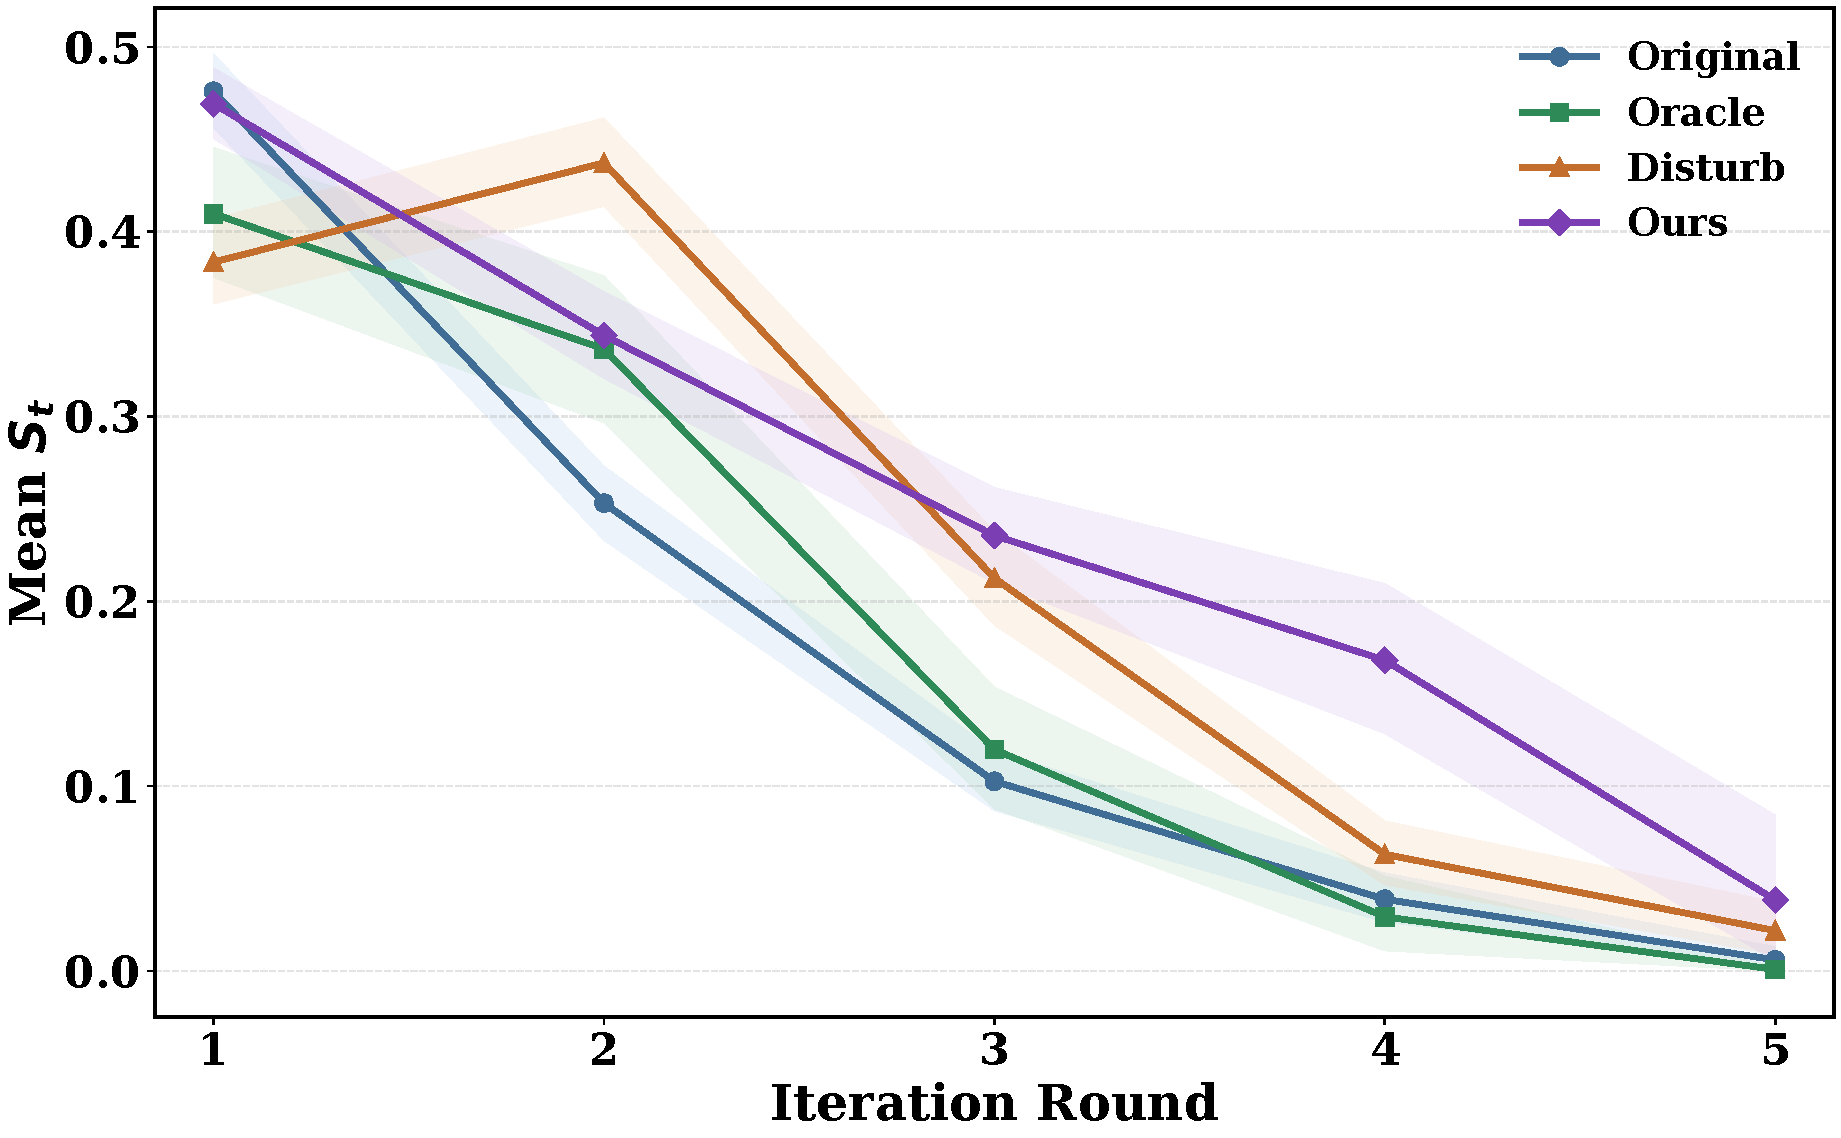
\includegraphics[width=0.9\linewidth]{refamb_ours_main_step_score_curve_with_baselines.pdf}
    \caption{Comparison of trajectory inactivation degree among IIGCR, two intervention modes, and the original pipeline.}
    \label{fig:refamb_ours_main_step_score_curve_with_baselines}
\end{figure}
\section{Theoretical Analysis on RTE}
\begin{proposition}
    $\mathrm{RTE}\in\left[0,1\right]$.
\end{proposition}
\begin{proof}
    We first analyze boundness of $S_t$. According to \eqref{eq:delta_f}, \eqref{eq:s_t},
    \begin{equation}
        \df=\frac{|\facts_t \cup \facts_{<t}|}{|\facts_t|+\epsilon} - \frac{|\facts_{<t}|}{|\facts_t|+\epsilon}\leq \frac{|\facts_t| + |\facts_{<t}|}{|\facts_t|+\epsilon}-\frac{|\facts_{<t}|}{|\facts_t|+\epsilon}.
    \end{equation}
    Besides,
    \begin{equation}
        |\facts_t \cup \facts_{<t}|-|\facts_{<t}|\geq 0,
    \end{equation}
    that is,
    \begin{equation}
        0\leq \df\leq \frac{|\facts_t|}{|\facts_t|+\epsilon}\leq 1.
    \end{equation}
    Also, 
    \begin{align}
        0\leq U_t\leq 1,
        0\leq G_t\leq 1
    \end{align}
    Thus, $0\leq S_t\leq 1$, hence $0\leq \mathrm{RTE}\leq 1$. And $\mathrm{RTE}=1$ iff 
    \begin{equation}
        \forall \tau\in\mathcal{T},U(\tau)=1\land \facts_\tau\cap\facts_{\tau-1}=\varnothing,
    \end{equation}
    $\mathrm{RTE}=0$ iff 
    \begin{equation}
        \forall \tau \in\mathcal{T},U(\tau)=0\lor \facts_\tau\subset\facts_{\tau-1}.
    \end{equation}
\end{proof}
% \begin{proposition}
%     \textbf{(Monotonic Penalty of Low‑Gain Retrieval).} Given fixed $U_t$ and $|\facts_t|$, As the number of new facts $|F|$ decreases, $S_t$ is non‑increasing monotonically.
% \end{proposition}
% \begin{proof}
%     Let $\forall \tau>\tau_k, k\in\left\{1,2,\dots|\mathcal{T}|\right\}$,$|F_{\tau+1}|<|F_\tau|$, and $U_{\tau+1}=U_\tau=U,G_{\tau+1}=G_\tau=G$,
%     \begin{align}
%         S_{\tau+1}-S_\tau&=U\cdot G\left[\frac{|\facts_{\tau+1} \cup \facts_{<\tau+1}|-|\facts_{<\tau+1}|}{|\facts_{\tau+1}|+\epsilon}-\frac{|\facts_{\tau} \cup \facts_{<\tau}|-|\facts_{<\tau}|}{|\facts_{\tau}|+\epsilon}\right]\\
%         &= U\cdot G\left[\frac{|\facts_{\tau+1} \cup \facts_{<\tau+1}|}{|\facts_{\tau+1}|+\epsilon}-\frac{|\facts_{\tau} \cup \facts_{<\tau}|}{|\facts_{\tau}|+\epsilon}\right]\\
%         &< U\cdot G\cdot\frac{|\facts_{\tau+1} \cup \facts_{<\tau+1}|-|\facts_{\tau} \cup \facts_{<\tau}|}{|\facts_{\tau}|+\epsilon}\\
%         &= U\cdot G\cdot \frac{|\facts_{\tau+1}| + |\facts_{\leq\tau}|-|\facts_{\tau+1}\cap \facts_{\leq\tau}|-|\facts_{\leq\tau}|}{|\facts_{\tau}|+\epsilon}
%     \end{align}
% \end{proof}
\begin{proposition}[\textbf{Monotonicity with Respect to New-Fact Ratio}]
Assume that the utility term $U_t$ and the grounding term $G_t$ remain fixed across two consecutive retrieval steps. Let
\[
\rho_t =
\frac{|F_t\setminus F_{<t}|}{|F_t|+\epsilon}
\]
denote the proportion of newly introduced facts in the retrieved fact set at step $t$. 
If $\rho_{\tau+1}\le \rho_{\tau}$, then the step score
\[
S_t = U_tG_t\rho_t
\]
is non-increasing, i.e.,
\[
S_{\tau+1}\le S_{\tau}.
\]
\end{proposition}

\begin{proof}
Under the fixed $U_t=U$ and $G_t=G$, the score difference between two consecutive retrieval steps is
\[
S_{\tau+1}-S_{\tau}
=
UG(\rho_{\tau+1}-\rho_{\tau}).
\]
Since $\rho_{\tau+1}\le \rho_{\tau}$ and $UG\ge 0$, we have
\[
S_{\tau+1}-S_{\tau}\le 0.
\]
Therefore, $S_{\tau+1}\le S_{\tau}$.
\end{proof}
\section{Case Study}
\subsection{Disturb Intervention}
As shown in Figure~\ref{fig:case_study_disturb} and Figure~\ref{fig:case_study_original}, the benefit of Disturb does not necessarily come from retrieving cleaner evidence.
After the first query is made referentially ambiguous, the retrieved documents become broader and noisier; however, this broader retrieval context can cause the VLM to restate the task objective more explicitly and decompose the comparison into two single-entity evidence-seeking steps.
The agent then retrieves the relevant facts separately and aggregates them into the final answer.
In contrast, the Original trajectory begins with a more explicit joint query, but the retrieved evidence fails to support both entities at once, which leads to a longer evidence-aggregation loop.
This case illustrates the main point of the paper: controlled ambiguity can alter the retrieval policy, but the resulting effect depends on whether the backbone uses that shift productively.
\begin{figure}[htbp]
    \centering
    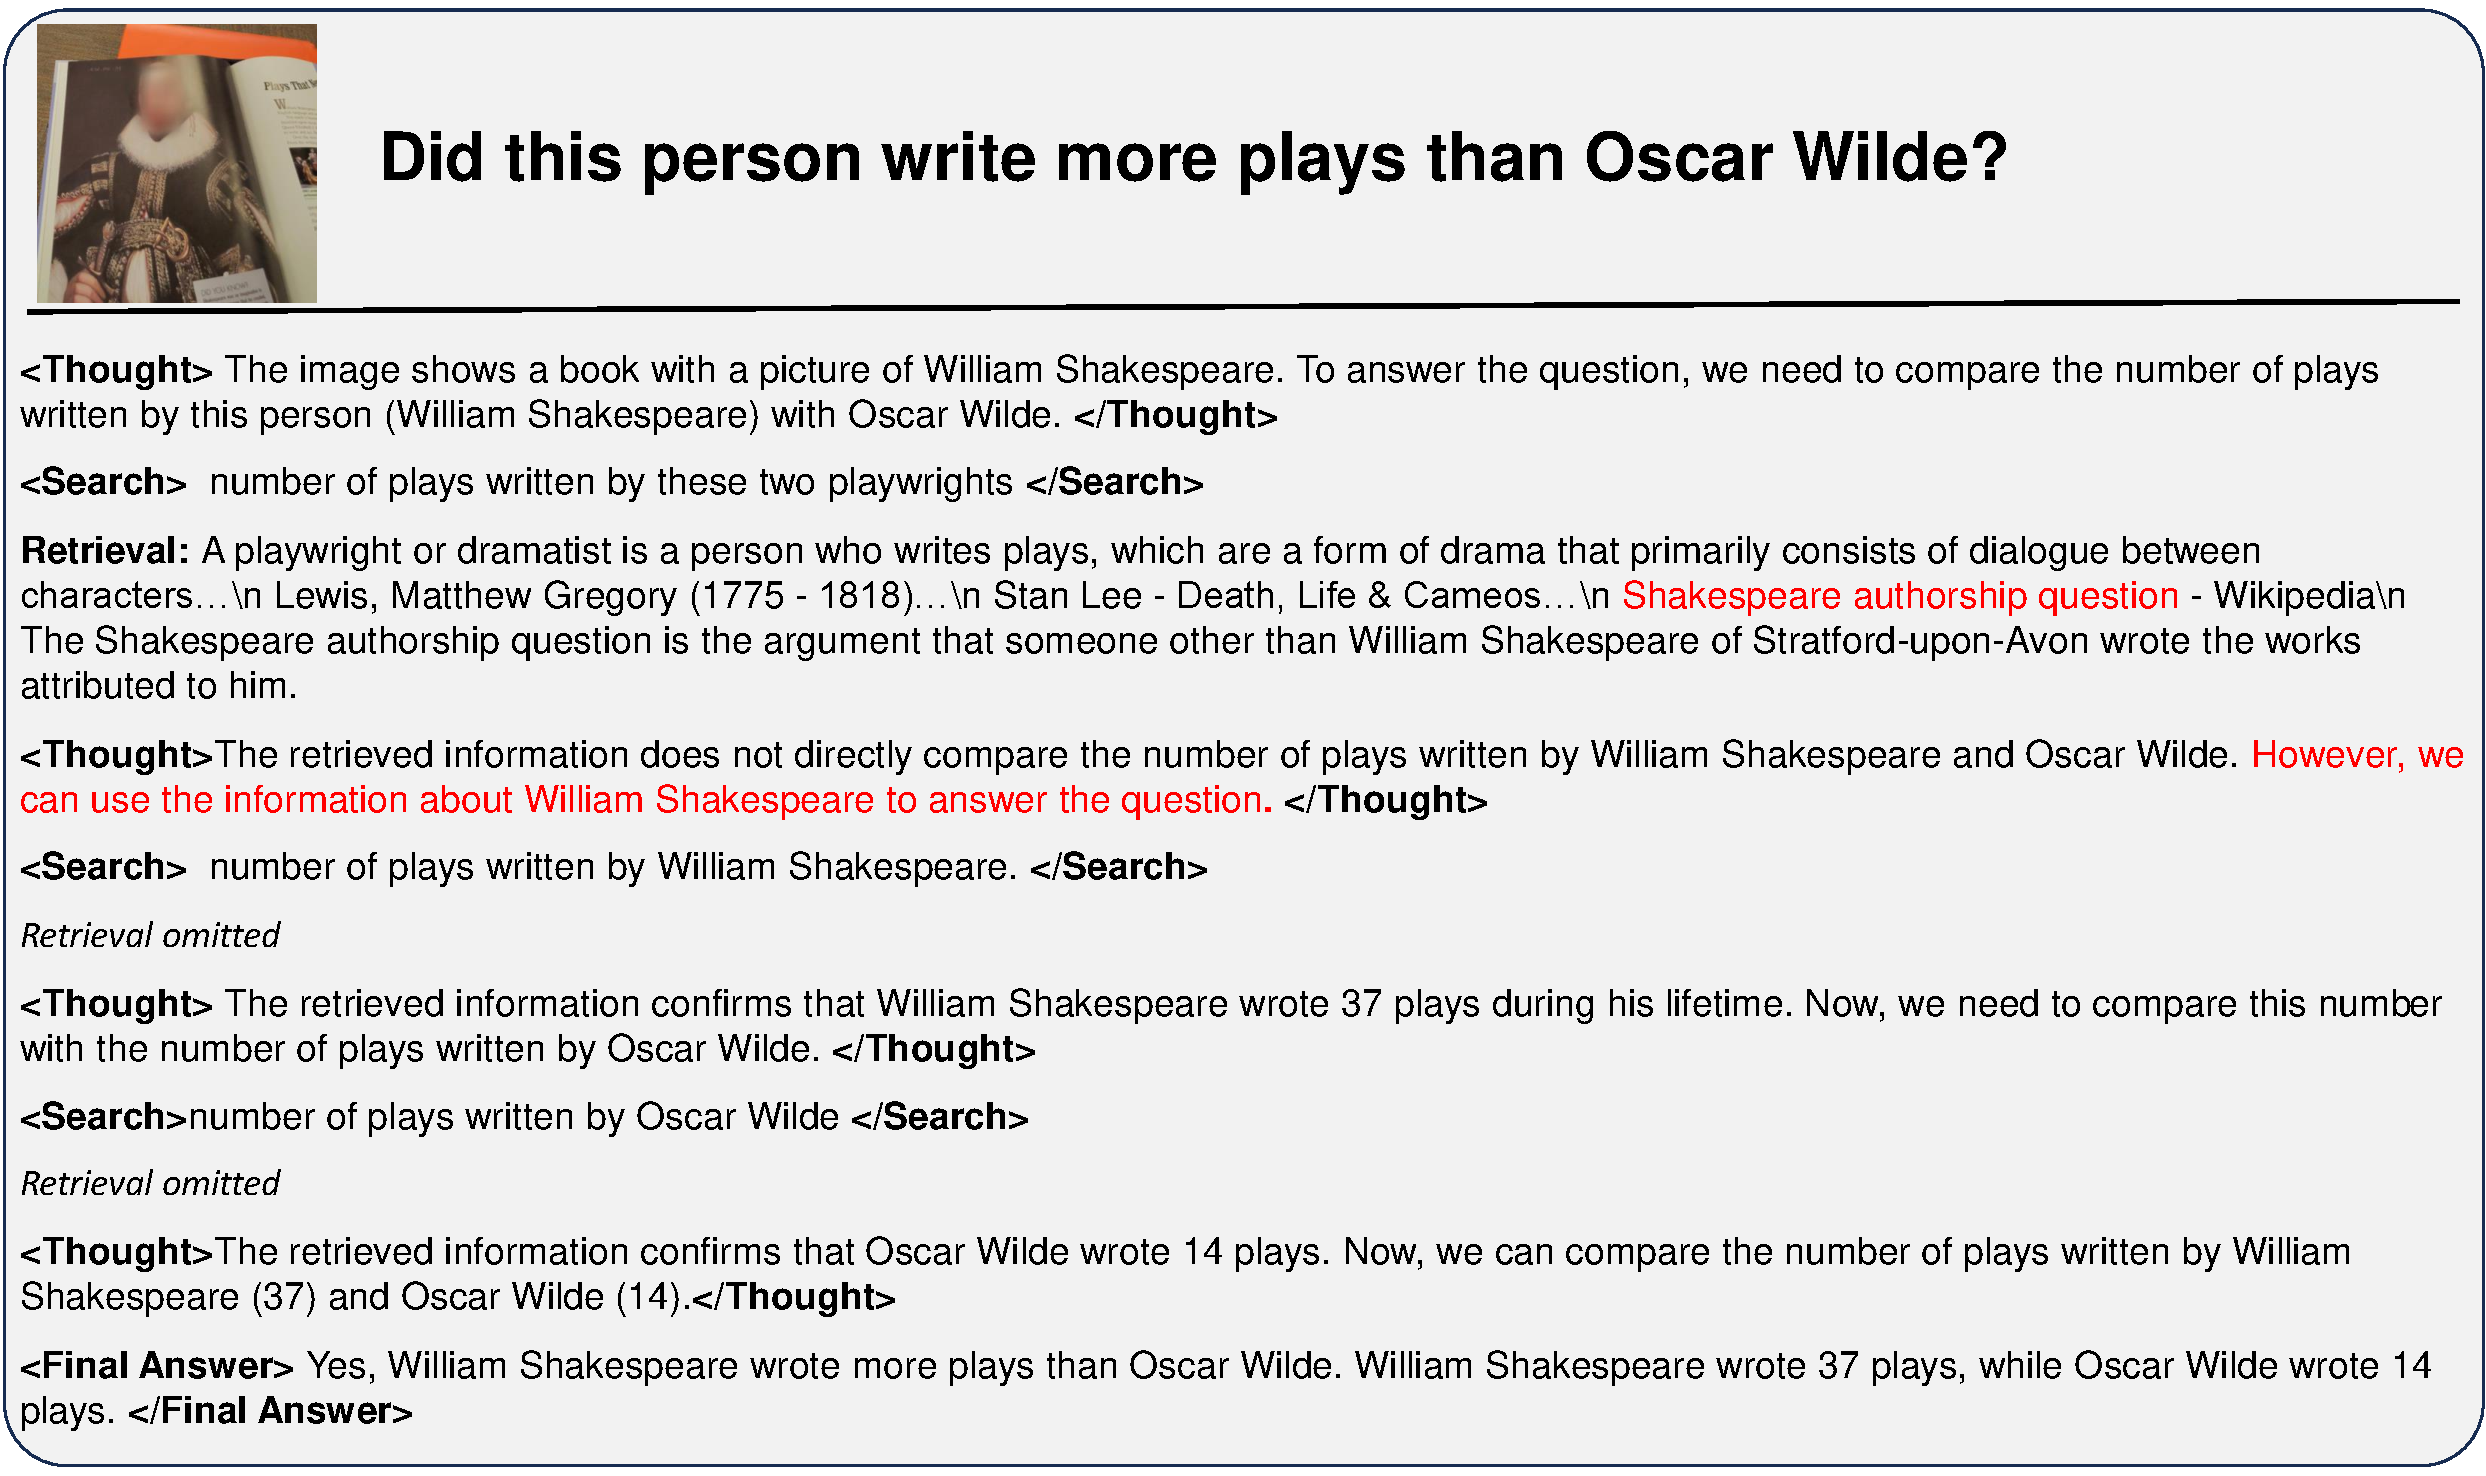
\includegraphics[width=\linewidth]{case_study_disturb.pdf}
    \caption{A case where Disturb changes the retrieval policy and leads to the correct final answer. The intermediate retrieval results are omitted.}
    \label{fig:case_study_disturb}
\end{figure} 
\begin{figure}[htbp]
    \centering
    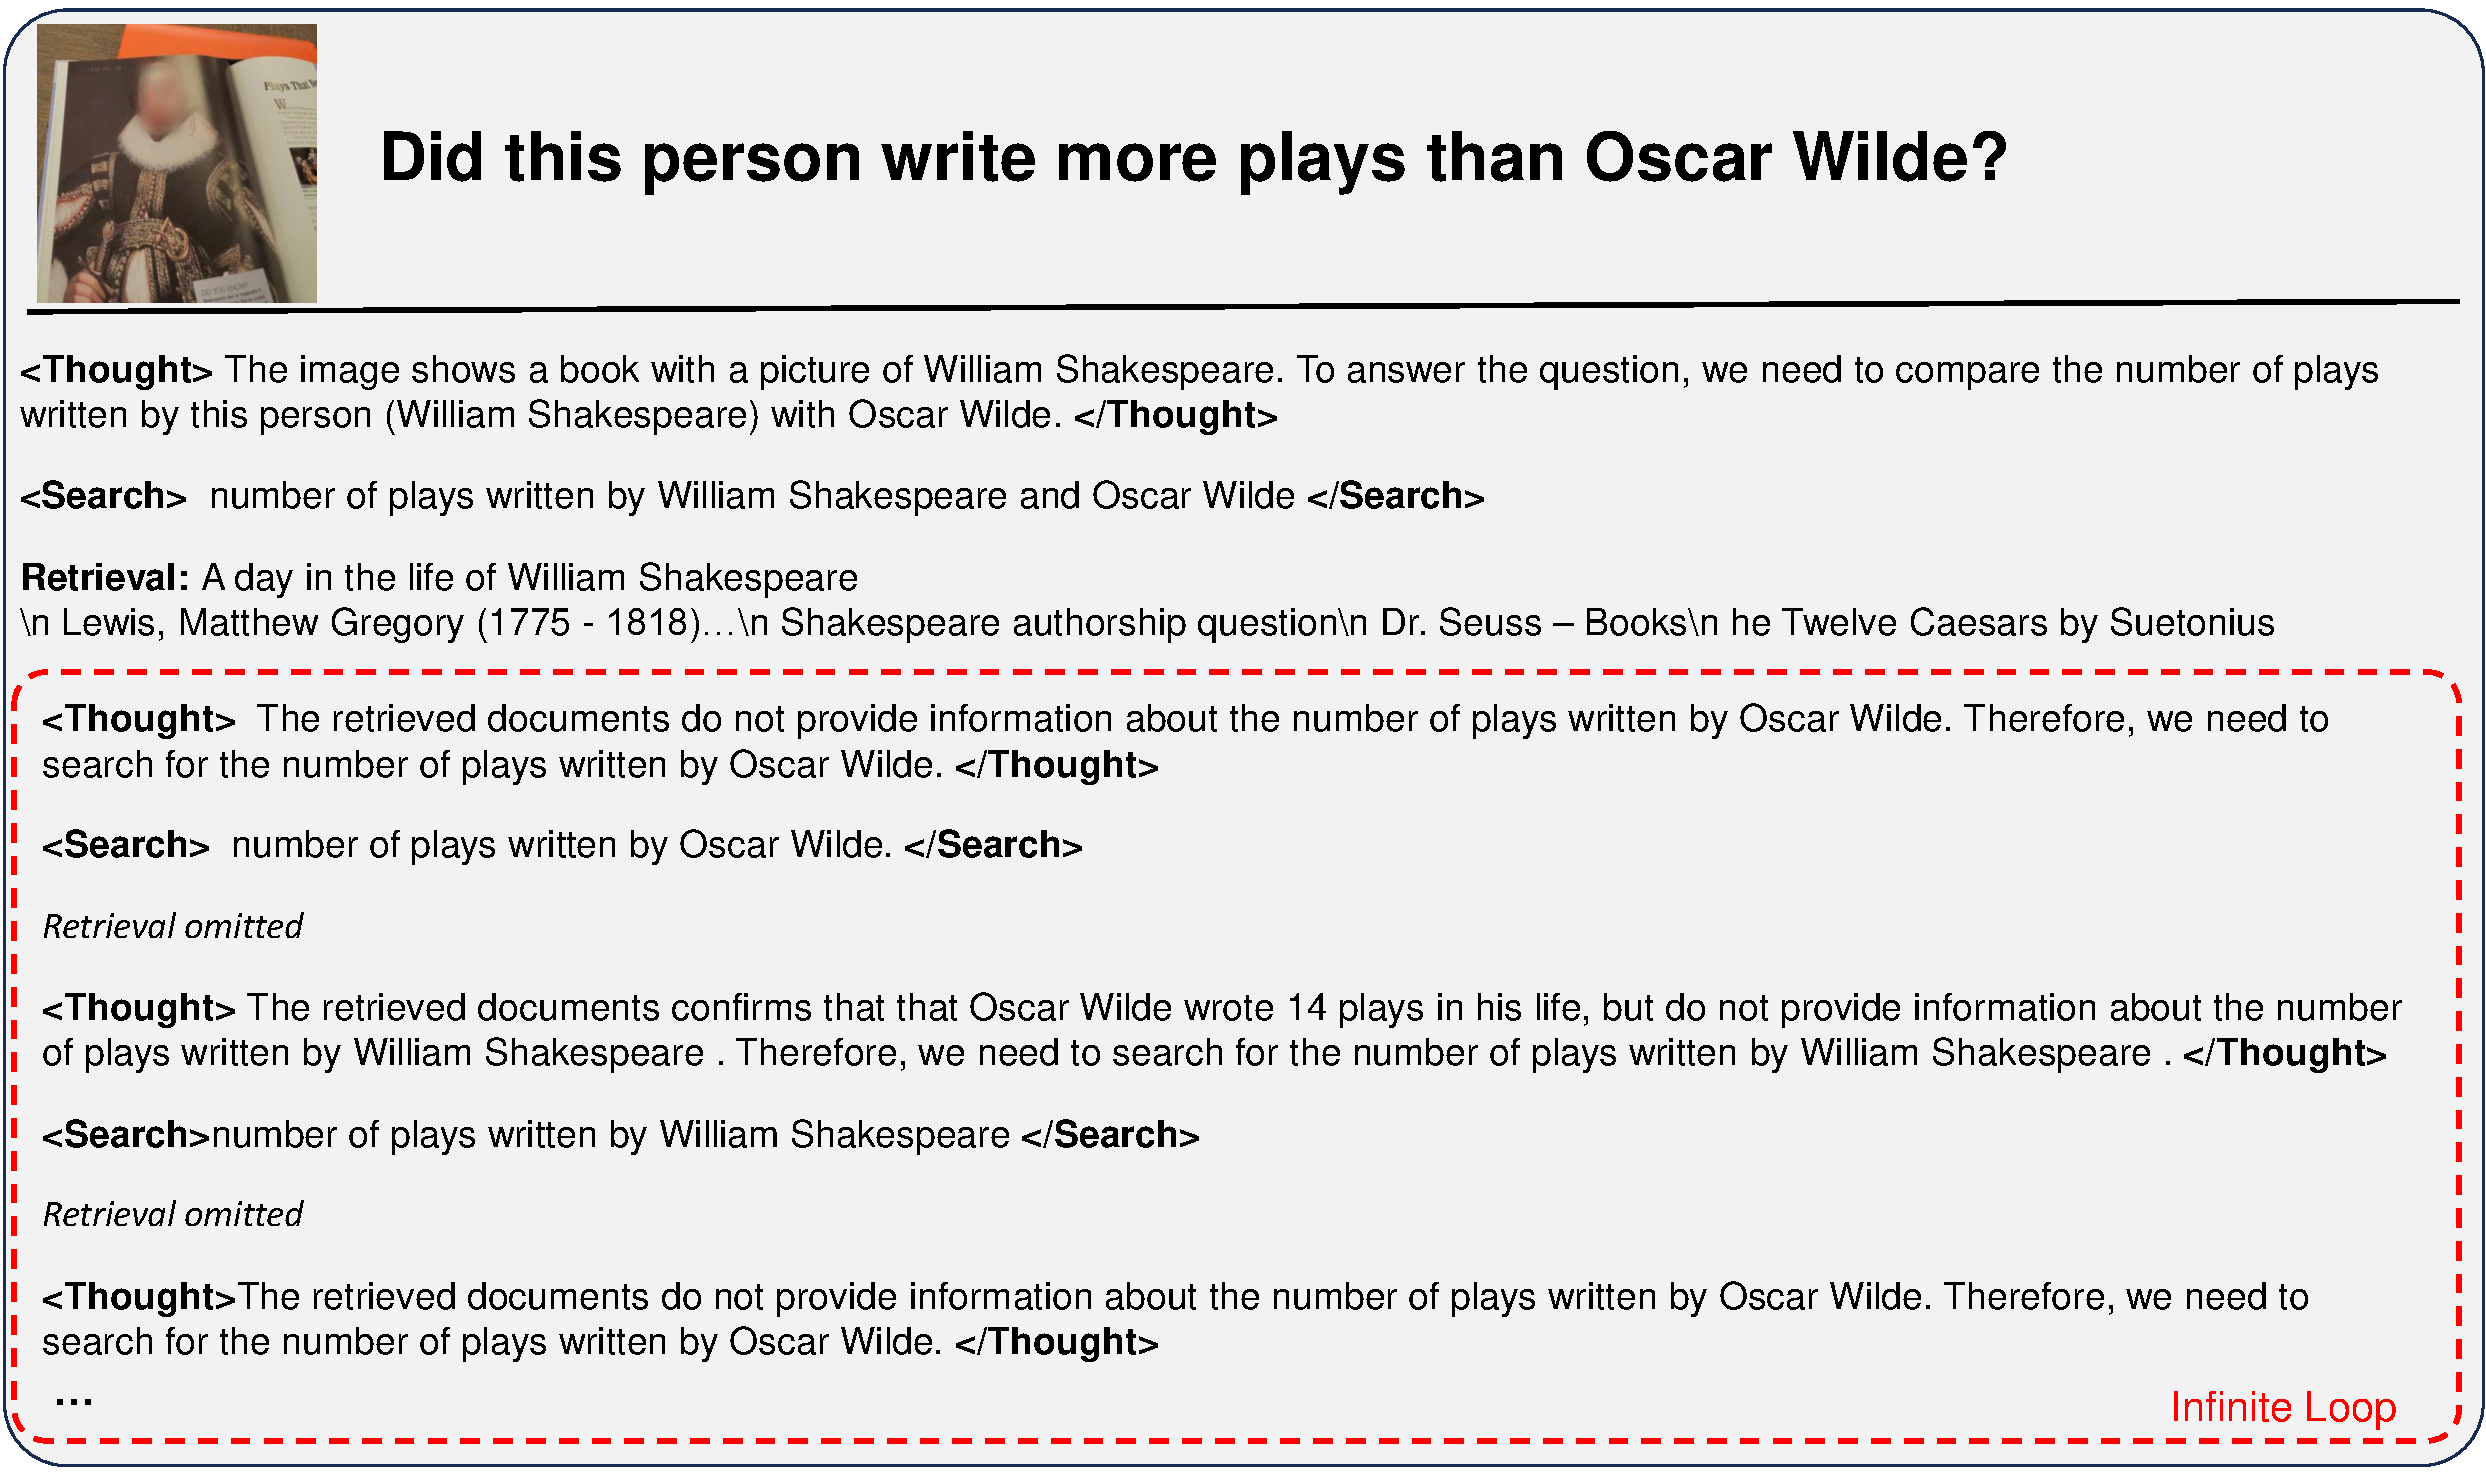
\includegraphics[width=\linewidth]{case_study_original.pdf}
    \caption{The trajectory before Disturb. The question is explicit, but the model still fails to aggregate evidence effectively.}
    \label{fig:case_study_original}
\end{figure}

\section{Limitations \& Future Work}
Although we now validate across several backbones, our results still do not establish a backbone-invariant law of query control.
The strongest positive effects remain concentrated in Qwen2.5-VL-7B and a subset of entity-centric settings, while Qwen3-family backbones often respond differently to the same rewrite.
As a result, the findings should be read as evidence for a controllability gap rather than as a universal recipe for repair.
Because API cost and runtime budget make a full specificity sweep impractical on the full 1,500-item benchmark, we rely on cross-backbone transfer, paired bootstrap, and stratified ambiguity bins as boundary checks instead of a dense intervention grid.
We have also not yet fully explained why some backbones convert canonical grounding into better trajectories while others do not.
That question likely depends on the interaction between retrieval policy, reasoning style, and the model's internal preference for exploration versus grounding.
Finally, evaluating retrieval quality in agentic trajectories remains intrinsically challenging.
Unlike static RAG settings where a question can sometimes be paired with pre-annotated golden evidence, ReAct-style pipelines generate retrieval queries dynamically, and the required evidence depends on the model's evolving sub-questions, intermediate beliefs, and previous retrieval feedback.
Even when dataset-level evidence annotations are available, they may not define step-level golden evidence for arbitrary agent-generated queries.
Future work should therefore develop more principled evaluation protocols for agentic retrieval, where the notion of supporting evidence is defined relative to dynamically generated queries and evolving reasoning states rather than assumed to be fixed at the question level.
Another promising direction is end-to-end joint training of large models and retrievers via reinforcement learning, where fine-grained signals about referential ambiguity, retrieval evidence utility, and trajectory-level information gain could guide the model toward query expressions that are both retrieval-aware and backbone-robust.
\section{Prompt Engineering}
\begin{tcolorbox}[
  title=Example: Entity Ambiguity Annotation Prompt,
  coltitle=black,
  colbacktitle=blue!8,
  colback=blue!5,
  colframe=black,
  fonttitle=\bfseries,
  arc=2mm,
  boxrule=0.5pt,
  enhanced jigsaw,
  breakable,
  width=\linewidth,
  left=6pt,
  right=6pt,
  top=6pt,
  bottom=6pt
]

\textbf{Input Prompt:}

\begin{itemize}
  \item Text Query: \texttt{\{text\_query\}}
\end{itemize}

\textbf{Task:}
Judge whether the query is \emph{entity-ambiguous} at the query-retriever interface.
The retriever only sees the text query, not the image or hidden context.

\textbf{Decision rule:}
Mark \texttt{"entity\_ambiguous": "Yes"} if the query does not uniquely specify the intended entity for retrieval.
Mark \texttt{"entity\_ambiguous": "No"} if the query already names a concrete retrievable target.
Do not confuse answer difficulty with entity ambiguity.

\textbf{Typical \texttt{Yes} cases:}
\begin{itemize}
  \item pronouns or deictic references such as ``it'', ``this'', or ``that'' when only the image resolves the referent;
  \item image-dependent phrases such as ``in the image'' or ``shown in the picture'';
  \item generic descriptions that could match many entities.
\end{itemize}

\textbf{Typical \texttt{No} cases:}
\begin{itemize}
  \item ``Address of Notre-Dame de Paris''
  \item ``When was Birkenstock founded?''
  \item ``temperature in Tillamook''
\end{itemize}

\textbf{Output format:}

\verb|{"entity_ambiguous": "Yes" or "No", "remark": ""}|
\end{tcolorbox}
\newpage
\begin{tcolorbox}[
  title=Example: Iteration Utility Annotation Prompt,
  coltitle=black,
  colbacktitle=blue!8,
  colback=blue!5,
  colframe=black,
  fonttitle=\bfseries,
  arc=2mm,
  boxrule=0.5pt,
  enhanced jigsaw,
  breakable,
  width=\linewidth,
  left=6pt,
  right=6pt,
  top=6pt,
  bottom=6pt
]

\textbf{Input Prompt:}

\begin{itemize}
  \item Sub-question: \texttt{\{sub\_question\}}
  \item Next Reasoning Text: \texttt{\{reasoning\}}
\end{itemize}

\textbf{Task:}
Judge how the retrieval result contributes to the model's next-step reasoning.
Return exactly one utility label for the current iteration.

\textbf{Allowed labels:}
\begin{itemize}
  \item \texttt{no\_contribution}
  \item \texttt{partial\_contribution}
  \item \texttt{full\_contribution}
\end{itemize}

\textbf{Decision rule:}
\begin{itemize}
  \item Use \texttt{no\_contribution} if the reasoning says the evidence is irrelevant, uninformative, insufficient, or discarded.
  \item Use \texttt{partial\_contribution} if the evidence helps only part of the sub-question, narrows the search, or resolves one component.
  \item Use \texttt{full\_contribution} if the evidence fully resolves the sub-question for this step.
  \item Judge from the model's own next reasoning text, not from your independent opinion.
\end{itemize}

\textbf{Contrastive cases:}
\begin{itemize}
  \item ``The documents do not provide information about X'' $\rightarrow$ \texttt{no\_contribution}
  \item ``The documents identify A, but not B'' $\rightarrow$ \texttt{partial\_contribution}
  \item ``According to the documents, the answer is X'' $\rightarrow$ \texttt{full\_contribution}
\end{itemize}

\textbf{Output format:}

\verb|{"label": "no_contribution", "reason": ""}|
\end{tcolorbox}

\begin{tcolorbox}[
  title=Example: InfoSeek Three-way Annotation Prompt,
  coltitle=black,
  colbacktitle=blue!8,
  colback=blue!5,
  colframe=black,
  fonttitle=\bfseries,
  arc=2mm,
  boxrule=0.5pt,
  enhanced jigsaw,
  breakable,
  width=\linewidth,
  left=6pt,
  right=6pt,
  top=6pt,
  bottom=6pt
]

\textbf{Input Prompt:}

\begin{itemize}
  \item Text Query: \texttt{\{text\_query\}}
  \item Image Query: \texttt{\{image\_query\}}
\end{itemize}

\textbf{Task:}
Assign exactly one label based on both the text and image query.
Do not answer the question itself.

\textbf{Label set:}
\begin{itemize}
  \item \texttt{Entity Recognition}
  \item \texttt{Single-hop Attribute Query}
  \item \texttt{Comparison}
\end{itemize}

\textbf{Decision rule:}
\begin{itemize}
  \item Use \texttt{Entity Recognition} when the main goal is to identify the depicted entity itself at a specific enough identity level.
  \item Use \texttt{Single-hop Attribute Query} when the entity is grounded, but the question asks for one direct fact, attribute, or relation about it.
  \item Use \texttt{Comparison} when the main goal is to compare two entities, attributes, or states.
\end{itemize}

\textbf{Output format:}

\verb|{"coarse_label": "...", "rationale": "...", "confidence": 0}|
\end{tcolorbox}

\begin{tcolorbox}[
  title=Example: $C_1$ Text-Alone Entity Identification Prompt,
  coltitle=black,
  colbacktitle=blue!8,
  colback=blue!5,
  colframe=black,
  fonttitle=\bfseries,
  arc=2mm,
  boxrule=0.5pt,
  enhanced jigsaw,
  breakable,
  width=\linewidth,
  left=6pt,
  right=6pt,
  top=6pt,
  bottom=6pt
]

\textbf{Input Prompt:}

\begin{itemize}
  \item Question: \texttt{\{question\}}
\end{itemize}

\textbf{Task:}
Decide whether the core target entity can be reliably identified from the question text alone.

\textbf{Label set:}
\begin{itemize}
  \item \texttt{Yes}
  \item \texttt{Partially}
  \item \texttt{No}
\end{itemize}

\textbf{Decision rule:}
\begin{itemize}
  \item Use \texttt{Yes} if the question text explicitly names the entity or gives enough information to reliably identify it.
  \item Use \texttt{Partially} if the text gives some descriptive clues, but not enough to uniquely identify the entity for retrieval.
  \item Use \texttt{No} if the text alone does not provide usable information to identify the entity.
\end{itemize}

\textbf{Output format:}

\verb|{"focused_entity": "...", "text_alone_identifies_entity": "...", "rationale_1": "...", "confidence": 0}|
\end{tcolorbox}

\begin{tcolorbox}[
  title=Example: $C_2$ External Evidence Dependency Prompt,
  coltitle=black,
  colbacktitle=blue!8,
  colback=blue!5,
  colframe=black,
  fonttitle=\bfseries,
  arc=2mm,
  boxrule=0.5pt,
  enhanced jigsaw,
  breakable,
  width=\linewidth,
  left=6pt,
  right=6pt,
  top=6pt,
  bottom=6pt
]

\textbf{Input Prompt:}

\begin{itemize}
  \item Question: \texttt{\{question\}}
  \item Gold Final Answer: \texttt{\{gold\_answer\}}
  \item Stage-1 Visual Evidence: \texttt{\{evidence\}}
\end{itemize}

\textbf{Task:}
Judge whether the final answer is uniquely recoverable from the image evidence alone.

\textbf{Label set:}
\begin{itemize}
  \item \texttt{Yes}
  \item \texttt{No}
  \item \texttt{Uncertain}
\end{itemize}

\textbf{Decision rule:}
\begin{itemize}
  \item Use \texttt{Yes} if the image evidence alone is sufficient to recover the final answer.
  \item Use \texttt{No} if the evidence is compatible with the answer but not sufficient to uniquely determine it, or if the answer requires evidence beyond the image.
  \item Use \texttt{Uncertain} if the evidence summary is incomplete or ambiguous enough that a confident decision cannot be made.
\end{itemize}

\textbf{Output format:}

\verb|{"answer_recoverable_from_image_alone": "...", "external_evidence_dependency": "...", "missing_information_type": [], "rationale": "...", "confidence": 0}|
\end{tcolorbox}

\begin{tcolorbox}[
  title=Example: C2 Stage-1 Visual Evidence Extraction Prompt,
  coltitle=black,
  colbacktitle=blue!8,
  colback=blue!5,
  colframe=black,
  fonttitle=\bfseries,
  arc=2mm,
  boxrule=0.5pt,
  enhanced jigsaw,
  breakable,
  width=\linewidth,
  left=6pt,
  right=6pt,
  top=6pt,
  bottom=6pt
]

\textbf{Input Prompt:}

\begin{itemize}
  \item Question: \texttt{\{question\}}
\end{itemize}

\textbf{Task:}
Extract only the task-relevant evidence that is directly observable in the image.
Do not answer the question.

\textbf{Output format:}

\verb|{"relevant_visible_evidence": [], "uncertain_or_missing_visual_points": [], "extractor_summary": "", "confidence": 0}|
\end{tcolorbox}

\begin{tcolorbox}[
  title=Example: LLM as Judge Prompt,
  coltitle=black,
  colbacktitle=blue!8,
  colback=blue!5,
  colframe=black,
  fonttitle=\bfseries,
  arc=2mm,
  boxrule=0.5pt,
  enhanced jigsaw,
  breakable,
  width=\linewidth,
  left=6pt,
  right=6pt,
  top=6pt,
  bottom=6pt
]

\textbf{Input Prompt:}

\begin{itemize}
  \item Reference Answers: \texttt{\{golden\_answers\}}
  \item Candidate's Answer: \texttt{\{pred\}}
\end{itemize}

\textbf{Task:}
Compare the candidate answer against the reference answers and judge whether it is semantically correct.

\textbf{Decision rule:}
\begin{itemize}
  \item Output \texttt{yes} if the candidate answer matches the reference meaning, even if wording differs.
  \item Output \texttt{no} if the answer is wrong, unsupported, incomplete, irrelevant, empty, or does not directly answer the question.
  \item Output exactly one token: \texttt{yes} or \texttt{no}.
\end{itemize}

\textbf{Output format:}

\verb|yes / no|
\end{tcolorbox}

\begin{tcolorbox}[
  title=Example: System VLM Prompt,
  coltitle=black,
  colbacktitle=blue!8,
  colback=blue!5,
  colframe=black,
  fonttitle=\bfseries,
  arc=2mm,
  boxrule=0.5pt,
  enhanced jigsaw,
  breakable,
  width=\linewidth,
  left=6pt,
  right=6pt,
  top=6pt,
  bottom=6pt
]

\textbf{Input Prompt:}

\begin{itemize}
  \item Input Question: \texttt{\{question\}}
\end{itemize}

\textbf{Task:}
Decompose the question into sub-questions and solve them step by step.
Use \texttt{Search} for retrieval and \texttt{Final Answer} only when the response is ready.

\textbf{Search actions:}
\begin{itemize}
  \item \texttt{Image Retrieval}: use an anchored phrase for the entity in the image.
  \item \texttt{Text Retrieval}: use a specific query for missing context.
  \item \texttt{No Retrieval}: if retrieval is unnecessary.
\end{itemize}

\textbf{Output format:}

Use the XML structure with \texttt{<Thought>}, \texttt{<Sub-Question>}, \texttt{<Search>}, and \texttt{<End>}.
\end{tcolorbox}

\begin{tcolorbox}[
  title=Example: Rewrite Similar Text Query Prompt,
  coltitle=black,
  colbacktitle=blue!8,
  colback=blue!5,
  colframe=black,
  fonttitle=\bfseries,
  arc=2mm,
  boxrule=0.5pt,
  enhanced jigsaw,
  breakable,
  width=\linewidth,
  left=6pt,
  right=6pt,
  top=6pt,
  bottom=6pt
]

\textbf{Input Prompt:}

\begin{itemize}
  \item Query To Rewrite: \texttt{\{query\_to\_rewrite\}}
  \item Feedback: \texttt{\{vlm\_feedback\}}
\end{itemize}

\textbf{Task:}
Recover from a blocked retrieval step by choosing a genuinely new retrieval action.
Do not repeat the previous query or produce a near-duplicate paraphrase.

\textbf{Decision rule:}
\begin{itemize}
  \item Use \texttt{Text Retrieval} only if a materially different query is justified.
  \item Use \texttt{Image Retrieval} if the missing clue must be grounded in the image.
  \item Use \texttt{No Retrieval} if retrieval is no longer useful.
\end{itemize}

\textbf{Output format:}

Use exactly one \texttt{<Search>} block.
\end{tcolorbox}
\newpage
\begin{tcolorbox}[
  title=Example: Alignment Layer Prompt,
  coltitle=black,
  colbacktitle=blue!8,
  colback=blue!5,
  colframe=black,
  fonttitle=\bfseries,
  arc=2mm,
  boxrule=0.5pt,
  enhanced jigsaw,
  breakable,
  width=\linewidth,
  left=6pt,
  right=6pt,
  top=6pt,
  bottom=6pt
]

\textbf{Input Prompt:}

\begin{itemize}
  \item Original Query: \texttt{\{original\_query\}}
  \item Enhanced Information: \texttt{\{enhanced\_information\}}
\end{itemize}

\textbf{Task:}
Rewrite the original query with grounded evidence so the new query is easier to retrieve.
Resolve ambiguous references, add only useful grounded details, and stay conservative when evidence is weak.

\textbf{Output format:}

\begin{itemize}
  \item \texttt{ambiguous\_references}
  \item \texttt{grounding\_cues}
  \item \texttt{entity\_status}
  \item \texttt{canonical\_entity}
  \item \texttt{alternative\_entities}
  \item \texttt{entity\_confidence}
  \item \texttt{entity\_type}
  \item \texttt{target\_attribute}
  \item \texttt{refined\_queries}
\end{itemize}
\end{tcolorbox}

\begin{tcolorbox}[
  title=Example: Oracle Rewrite Prompt,
  coltitle=black,
  colbacktitle=blue!8,
  colback=blue!5,
  colframe=black,
  fonttitle=\bfseries,
  arc=2mm,
  boxrule=0.5pt,
  enhanced jigsaw,
  breakable,
  width=\linewidth,
  left=6pt,
  right=6pt,
  top=6pt,
  bottom=6pt
]

\textbf{Input Prompt:}

\begin{itemize}
  \item Original Question: \texttt{\{question\}}
  \item Original Text Query: \texttt{\{text\_query\}}
  \item Ambiguity Level: \texttt{\{ambiguity\_level\}}
  \item Answers: \texttt{\{answers\}}
\end{itemize}

\textbf{Task:}
Rewrite an entity-ambiguous retrieval query into an entity-explicit query grounded in the provided answers.
Preserve the original retrieval intent and keep edits minimal whenever possible.

\textbf{Decision rule:}
\begin{itemize}
  \item For object identification, output the canonical entity name only.
  \item For description or indirect ambiguity, replace the vague referent with the grounded entity name.
  \item For no-object-involved cases, keep translation queries unchanged when appropriate, otherwise disambiguate the target phrase using the answers.
  \item If the query is already explicit enough for text retrieval, return it unchanged.
\end{itemize}

\textbf{Output format:}

\verb|{"rewritten_query": ""}|
\end{tcolorbox}
\newpage
\begin{tcolorbox}[
  title=Example: Disturb Rewrite Prompt,
  coltitle=black,
  colbacktitle=blue!8,
  colback=blue!5,
  colframe=black,
  fonttitle=\bfseries,
  arc=2mm,
  boxrule=0.5pt,
  enhanced jigsaw,
  breakable,
  width=\linewidth,
  left=6pt,
  right=6pt,
  top=6pt,
  bottom=6pt
]

\textbf{Input Prompt:}

\begin{itemize}
  \item Query: \texttt{\{query\}}
\end{itemize}

\textbf{Task:}
Rewrite the query into a more referentially ambiguous version for a controlled perturbation experiment.
Preserve the original intent, answer target, and task type, but reduce referential clarity.

\textbf{Decision rule:}
\begin{itemize}
  \item Replace explicit entity names with vague referential expressions when possible.
  \item Keep the query close in length and structure to the original.
  \item Do not change the queried attribute, relation, event, or comparison target.
  \item If the query is already vague, keep it unchanged rather than making it broader.
\end{itemize}

\textbf{Output format:}

Return only the rewritten query.
\end{tcolorbox}
\end{document}
